%!TEX program = lualatex
%!TEX encoding = UTF-8 Unicode  
%!TEX root = chapter06.tex  
\documentclass[main.tex]{subfiles} 
\begin{document} 
%----------------------------------------------------------------------------------------
%	CHAPTER 6
%----------------------------------------------------------------------------------------
\cleardoublepage 
\loadgeometry{marginlayout}  
\pagestyle{scrheadings} % Print headers again  
\KOMAoptions{
headwidth=textwithmarginpar,
headsepline=true,
headsepline= 0.5pt,
footwidth=textwithmarginpar,
}   
\onehalfspacing 
\setcounter{chapter}{5}
\chapter{Figures semblables}

\section{Triangles semblables}



\begin{definition} Deux triangles sont \textbf{semblables} lorsqu'ils ont leurs angles égaux deux à deux et leurs côtés \textbf{proportionnels}. 
\end{definition}

\begin{figure}[h]\centering
	\begin{tikzpicture}[scale=0.75]
		\tkzDefPoint(0,0){A}
		\tkzLabelPoint[above left](A){$A$}
		\tkzDefShiftPoint[A](-135:2.5){B}  
		\tkzDefTriangle[two angles = 80 and 60](A,B)
		\tkzGetPoint{C}
		\tkzLabelPoint[left](B){$B$}
		\tkzLabelPoint[right](C){$C$}
		\tkzDrawPolygon(A,B,C)
		\tkzDrawPoints(A,B,C)
		\tkzDefShiftPoint[A](4,-0.5){J}  
		\tkzDefShiftPoint[J](10:6){I}
		\tkzDefTriangle[two angles = -60 and -40](I,J)
		\tkzGetPoint{K}
		\tkzDrawPolygon(I,J,K)
		\tkzDrawPoints(I,J,K) 
		\tkzLabelPoint[right](I){$I$}
		\tkzLabelPoint[left](J){$J$}
		\tkzLabelPoint[right](K){$K$}
		\tkzMarkAngle[mark=|,mkcolor=black, thick, size=0.6, fill=red!20, opacity=0.6](B,A,C)
		\tkzMarkAngle[mark=|,mkcolor=black, thick,size=0.6, fill=red!20, opacity=0.6](J,K,I)
		\tkzMarkAngle[mark=||,mkcolor=black, thick,size=0.6, fill=blue!20, opacity=0.6](A,C,B)
		\tkzMarkAngle[mark=||,mkcolor=black, thick,size=0.6, fill=blue!20, opacity=0.6](I,J,K) 
		\tkzMarkAngle[mark=s,mkcolor=black, thick,size=0.6, fill=green!20, opacity=0.6](C,B,A)
		\tkzMarkAngle[mark=s,mkcolor=black, thick,size=0.6, fill=green!20, opacity=0.6](K,I,J)
		\tkzDrawSegment[line width=2pt, color=red](B,C)
		\tkzDrawSegment[line width=2pt, color=red](I,J)
		\tkzDefMidPoint(B,C)\tkzGetPoint{D}
		\tkzDefMidPoint(I,J)\tkzGetPoint{L}
		\draw[<->, >=latex] (A) .. controls +(right:1cm) and +(left:2cm) .. (K) node[sloped,above,pos=0.5]{\scriptsize Angles homologues} ;
		\draw[<->, >=latex] (D) .. controls +(right:8cm) and +(down:4cm) .. (L) node[ below right,pos=0.6]{\scriptsize Côtés homologues} ;
	\end{tikzpicture}
	\caption{les trianges $ABC$ et $IJK$ sont semblables.}
\end{figure} 
\begin{enumerate}
	\item Les \textbf{angles homologues} sont égaux :
	%\[ \]
	\[{\color{red} \widehat{A}= \widehat{K} }\qquad {\color{blue} \widehat{B}= \widehat{J} }\qquad {\color{ForestGreen} \widehat{C}= \widehat{I} }\]
	
	\item Les \textbf{côtés correspondants} sont proportionnels  :    
	\begin{table}[h]
		\renewcommand{\arraystretch}{2}%
		\begin{tabularx}{0.9\linewidth}{|X?c|c|c|} \hline 
			\tikz[remember picture,baseline =(C.base)]\node (C) at (-1cm,0.5cm) {};	{\color{HotPink} Côtés  du triangle $ABC$} &  \emph{\color{blue}$AB$}&  \emph{\color{red}$BC$} & \emph{$AC$} \tikz[remember picture]   \node  (A) at (-1cm,0.5cm) {}; \\   \hline
			\tikz[remember picture,baseline =(D.base)]\node (D) at (-1cm,0.5cm) {};	{\color{ForestGreen} Côtés  du triangle $IJK$} &  \emph{\color{blue}$JK$}&  \emph{\color{red}$IJ$}& \emph{$IK$} \tikz[remember picture,baseline =(B.base)]\node (B) at (-1cm,0.5cm) {}; \\ \hline
		\end{tabularx}
		%	\tikz[overlay,remember picture]
		%	\draw[ ->,>=latex,line width=1.8pt ](A) .. controls +(+1.5cm,.1cm) and +(+1.5cm,-.0cm)..
		%	node[rectangle,fill=white,draw,circle ]{\Large$\times k$} (B);
		\tikz[overlay,remember picture]
		\draw[ ->,>=latex,line width=1.8pt ](C) .. controls +(-1.5cm,.1cm) and +(-1.5cm,-.0cm)..
		node[rectangle,fill=white,draw,circle ]{\Large$\times k$} (D);
		\caption{ Si $k> 1$, le triangle $IJK$ est un \emph{agrandissement} de $ABC$.
			Si $k< 1$, le triangle $IJK$ est une \emph{réduction} de $ABC$.}
	\end{table}
	%	\begin{center}
	%		\begin{tikzpicture}
	%			% Création du tableau dans un nœud
	%			\node[anchor=east,rectangle,inner sep=0pt,outer sep=0pt]%
	%			(Tbl) {%
	%				\renewcommand{\arraystretch}{2}%
	%				\begin{tabularx}{1.0\columnwidth}{|c?X|X|X|} \hline 
	%					{\color{HotPink} Longueurs des côtés  du triangle $ABC$} &  \emph{\color{blue}$AB$}&  \emph{\color{red}$BC$} & \emph{$AC$} \\ \hline \hline
	%					{\color{ForestGreen} Longueurs des côtés  du triangle $IJK$} &  \emph{\color{blue}$JK$}&  \emph{\color{red}$IJ$}& \emph{$IK$} \\ \hline
	%				\end{tabularx}	 %
	%			};
	%			
	%			% Positionnement des points d'ancrage des flèches
	%			\path (Tbl.north east) -- (Tbl.south east) %
	%			node[pos=0.25](Fl_C){}% départ flèche courbe
	%			node[pos=0.75](C_lF){}; % pointe flèche rectangulaire
	%			\path (Tbl.north west) -- (Tbl.south west) %
	%			node[pos=0.25](Fl_R){}% départ flèche rectangulaire
	%			node[pos=0.75](R_lF){};% pointe  flèche courbe
	%			%\path (Tbl.north west) -- (Tbl.north east) node[pos=..](<nom du nœud>){}
	%			
	%			% Flèche courbe
	%			\draw[->,line width=.8pt,blue!80](Fl_C) .. controls +(1.5cm,.1cm) and +(2.5cm,-.1cm)..
	%			node[ellipse,fill=white,draw ]{$\times k$} (C_lF);
	%		\end{tikzpicture}
	%	\end{center}
	
	%	$$ {\color{blue} \frac{AB}{JK} } =  \color{red} \frac{BC}{IJ}   =  \color{ForestGreen} \frac{AC}{IK}  = \color{black} {\frac{1}{k}}  
	%	$$
	$$	{\color{blue} \frac{JK}{AB} } = {\color{red} \frac{IJ}{BC} } = {\color{ForestGreen} \frac{IK}{AC} } \color{black} =k 	$$
	
	
	%	On peut écrire l'égalité des rapports suivants :	
	%	\[
	%	{\color{blue} \frac{AB}{JK}  =  \color{red} \frac{BC}{IJ}   =  \color{ForestGreen} \frac{AC}{IK}  = \color{black} {\frac{1}{k}} \qquad \text{ou encore} \qquad
	%		{\color{blue} \frac{JK}{AB} } = {\color{red} \frac{IJ}{BC} } = {\color{ForestGreen} \frac{IK}{AC} } \color{black} =k }
	%	\]
\end{enumerate}  
%----------------------------------------------------------------------------------------
%	 
%----------------------------------------------------------------------------------------

\section{Homothéties}
L’homothétie de centre $O$ et rapport $k$ est une transformation qui permet d’agrandir ou de réduire une figure. L’image produite est \textbf{semblable} à la figure de départ. 
\begin{cBox}[frametitle={cas rapport positif : $k>0$}]
Pour construire l'image $M'$ d'un point $M$ par rapport à l'homothétie de centre $O$ et de rapport $k>0$ il faut :
\begin{dingautolist}{192}
	\item tracer la droite $(OM)$
	\item mesurer la distance $OM$ puis calculer $OM'=k\times OM$
	\item reporter la longueur $OM'$ en plaçant $M'$ du \textbf{même côté}  que $M$ par rapport à $O$.
\end{dingautolist} 
\end{cBox}
\begin{example} 	Sur le dessin, $A'$ est l'image de $A$ par l’homothétie de centre $O$ et de rapport   $\numprint{2.5}$.
	\begin{enumerate}[label=\alph*),leftmargin=*]
		\item Dessine l'image de $B$ puis celle du quadrilatère par  cette homothétie.
		\item Dessine l'image de la figure obtenue par l'homothétie de centre $P$ et de rapport $\numprint{0.4}$
	\end{enumerate}
	\begin{figure*}[h]
		\begin{tikzpicture}%[scale=0.4]
			\tkzSetUpPoint[size=3, fill=black]
			\tkzfctset{tan style/.style={->,>=latex, color=red, line width=1.2pt}} 
			\tkzInit[ymin=-5,ymax=5.5,xmin=-1,xmax=25]
			\tkzClip
			\tkzDefPoint(1.144,-0.2){O}
			\tkzDefPoint(16.0,+0.4){O'}
			\tkzDefPoint(2.96, 0.55){A1}
			\tkzDefPoint(3.04, -1.24){A2}
			\tkzDefPoint(4.8, -0.24){A3}
			\tkzDefPoint(4.0, 1.4){A4} 
			\tkzFillPolygon[color=Cyan!50](A1,A2,A3,A4)
			\foreach \i in {1,2,3,4}{%
				\tkzDefPointBy[homothety=center O ratio 2.5](A\i) \tkzGetPoint{B\i}
				\tkzDefPointBy[homothety=center O' ratio 0.4](B\i) \tkzGetPoint{C\i}
			}
			\tkzDrawPolygon[line width=2pt](A1,A2,A3,A4)
			%\tkzDrawPolygon[line width=1pt](B1,B2,B3,B4)
			%\tkzDrawPolygon[line width=1pt](C1,C2,C3,C4)
			%\tkzFillPolygon[color=HotPink!05](B1,B2,B3,B4)
			%\tkzFillPolygon[color=ForestGreen!05](C1,C2,C3,C4)
			\tkzDrawLines[add=0.2 and 0.2 , dashed ](O,B4)
			\tkzDrawLines[add=0.2 and 0.2 , dashed ](O,B3)
			%\foreach \i in {1,2,3,4}{
			%\tkzDrawLines[add=0.2 and 0.2 , dashed ](O,B\i)
			%}
			\foreach \i in {1,2,3,4}{
				\tkzDrawPoints[color=blue, size=5, fill=white](A\i)
				\tkzDrawPoints[color=blue, size=5, fill=white](B4)
				%\tkzDrawPoints[color=blue, size=1, fill=white](B\i)
				%\tkzDrawPoints[color=blue, size=1, fill=white](C\i)
			}
			\tkzDrawPoints[color=blue, size=5, fill=white](B4)
			\tkzDrawPoints[shape=cross,color=blue, size=15](O)
			\tkzDrawPoints[shape=cross,color=blue, size=15, fill=white](O')
			\tkzLabelPoint[above](O){$O$}
			\tkzLabelPoint[above](O'){$P$} 
			\tkzLabelPoint[above](A4){$A$}
			\tkzLabelPoint[right](A3){$B$}
			\tkzLabelPoint[above](B4){$A'$}
			%\tkzLabelPoint[above](B3){$B'$}
			%\tkzLabelPoint[above](C4){$A''$}
			\foreach \i in {1,2,3,4}{
				%\tkzLabelPoint(A\i){\footnotesize $A_\i$}
				%\tkzLabelPoint(B\i){\footnotesize $B_\i$}
				%\tkzLabelPoint(C\i){\footnotesize $C_\i$}
			}
		\end{tikzpicture}
	\end{figure*}
\end{example}


\newpage  
\begin{cBox}[frametitle={cas rapport négatif : $k<0$}]
Pour construire l'image $M'$ d'un point $M$ par rapport à l'homothétie de centre $O$ et de rapport $k$ il  faut :
\begin{dingautolist}{192}
	\item tracer la droite $(OM)$
	\item mesurer la distace $OM$ puis calculer $OM'=-k\times OM$
	\item reporter le point $M'$ est du \textbf{côté opposé} que $M$ par rapport à $O$.
\end{dingautolist} 
\end{cBox}
\begin{example} \hfill
	
	Sur la figure, le point $B_2$ est l'image de $A_2$ par l'homothétie de centre $O$ et de rapport $-3$.
	
	Dessine l'image de la figure bleue par les homothéties de centre $O$ et de rapports $-3$ et $\numprint{-1}$. 
	
	\begin{figure*}[h]
		\begin{tikzpicture}[scale=0.35]
			\tkzInit[ymin=-15,ymax=10.5,xmin=-30,xmax=15]
			\tkzClip
			\tkzDefPoint(2.86,-0.5){O}
			\tkzDefPoint(7.4, 1.68){A1}
			\tkzDefPoint(7.6, -3.1){A2}
			\tkzDefPoint(12.0, -0.6){A3}
			\tkzDefPoint(10.0, 3.5){A4}
			\tkzFillPolygon[color=Cyan!50](A1,A2,A3,A4)
			\foreach \i in {1,2,3,4}{%
				\tkzDefPointBy[homothety=center O ratio -3.0](A\i) \tkzGetPoint{B\i}
				\tkzDefPointBy[homothety=center O ratio -0.5](A\i) \tkzGetPoint{C\i}
			}
			\tkzDrawPolygon[line width=2pt](A1,A2,A3,A4)
			%\tkzDrawPolygon[line width=1pt](B1,B2,B3,B4)
			%\tkzDrawPolygon[line width=1pt](C1,C2,C3,C4)
			%\tkzFillPolygon[color=HotPink!05](B1,B2,B3,B4)
			%\tkzFillPolygon[color=ForestGreen!05](C1,C2,C3,C4)
			\foreach \i in {1,2,3,4}{
				\tkzDrawLines[add=0.2 and 0.1 , dashed ](A2,B2)
				%\tkzDrawLines[add=0.2 and 0.2 , dashed ](A\i,B\i)
			}
			\foreach \i in {1,2,3,4}{
				\tkzDrawPoints[color=blue, size=5, fill=white](A\i)
				\tkzDrawPoints[color=blue, size=5, fill=white](B2)
				%\tkzDrawPoints[color=blue, size=1, fill=white](B\i)
				%\tkzDrawPoints[color=blue, size=1, fill=white](C\i)
			}
			\tkzDrawPoints[shape=cross, color=blue, size=15, fill=white](O)
			\tkzLabelPoint[below left](O){$O$}
			\tkzLabelPoint[below](B2){$B2$}
			\foreach \i in {1,2,3,4}{
				\tkzLabelPoint(A\i){\footnotesize $A_\i$}
				%\tkzLabelPoint(B\i){\footnotesize $B_\i$}
				%\tkzLabelPoint(C\i){\footnotesize $C_\i$}
			}
		\end{tikzpicture}
	\end{figure*}
\end{example}


%----------------------------------------------------------------------------------------
%	 
%----------------------------------------------------------------------------------------

\newpage  
\section{Théorème de Thalès, la contraposée et sa réciproque}
Le théorème de Thalès est un cas particulier du critère de similitude AA qui s'applique à une situation ou les 2 triangles sont soit emboités soit opposés par un des sommets (en papillon). 


\begin{figure*}[tbp]\centering
	\begin{tikzpicture}[scale=0.8]
		\tkzSetUpPoint[size=3, fill=black]
		\tkzfctset{tan style/.style={->,>=latex, color=red, line width=1.2pt}}  
		\tkzInit[xmin=-1,xmax=4,ymin=-0.25,ymax=2.2,xstep=0.5, ystep=0.5];
		%\tkzSetUpLine[add=.5 and .5]
		\tkzDefPoints{0/0/B,3.0/0/C, -0.8/0/D, 4.3/0/E}
		\tkzDefTriangle[two angles=58 and 40](B,C)\tkzGetPoint{A}
		\tkzDrawPolygon[line width=1.2pt](A,B,C)
		\tkzDefPointWith[linear,K=0.55](A,B) \tkzGetPoint{P}
		\tkzDefPointWith[linear,K=0.75](A,C) \tkzGetPoint{Q}
		% \tkzDefPointWith[linear,K=-0.3](Q,P) \tkzGetPoint{P'}
		\tkzDrawLine[add=0.5 and 0.5 , line width=1.2pt](P,Q) 
		\tkzLabelPoints(C) 
		\tkzLabelPoints[below left](B) 
		\tkzLabelPoints[above](A)
		\tkzLabelPoints[above left](P) 
		\tkzLabelPoints[above right](Q) 
		% \tkzMarkAngle[mark=none,-, >=latex, size =0.7](P,A,Q)
		% \tkzLabelAngles[pos=1.0, fill = white](P,A,Q){$x$}
		% \tkzMarkAngle[mark=none,-, >=latex, size =0.65](A,B,D)
		% \tkzLabelAngles[pos=0.8, fill = white](A,B,D){$\ang{134}$}
		% \tkzMarkAngle[mark=none,-, >=latex, size =0.65](P',Q,A)
		% \tkzLabelAngles[pos=0.8, fill = white](P',Q,A){$\ang{132}$}
		\begin{scope}[xshift=10cm]
			\tkzDefPoints{0/0/B,3.5/0/C, -0.8/0/D, 4.3/0/E}
			\tkzDefTriangle[two angles=58 and 40](B,C)\tkzGetPoint{A}
			\tkzDrawPolygon[line width=1.2pt](A,B,C)
			\tkzDefPointWith[linear,K=-0.55](A,B) \tkzGetPoint{P}
			\tkzDefPointWith[linear,K=-0.75](A,C) \tkzGetPoint{Q}
			% \tkzDefPointWith[linear,K=-0.3](Q,P) \tkzGetPoint{P'}
			\tkzDrawLine[add=0.5 and 0.5 , line width=1.2pt](P,Q) 
			\tkzLabelPoints(C) 
			\tkzLabelPoints[below left](B) 
			\tkzLabelPoints[right](A)
			\tkzLabelPoints[above left](P) 
			\tkzLabelPoints[above right](Q) 
			\tkzDrawPolygon[line width=1.2pt](A,P,Q)
			% \tkzMarkAngle[mark=none,-, >=latex, size =0.7](P,A,Q)
			% \tkzLabelAngles[pos=1.0, fill = white](P,A,Q){$x$}
			% \tkzMarkAngle[mark=none,-, >=latex, size =0.65](A,B,D)
			% \tkzLabelAngles[pos=0.8, fill = white](A,B,D){$\ang{134}$}
			% \tkzMarkAngle[mark=none,-, >=latex, size =0.65](P',Q,A)
			% \tkzLabelAngles[pos=0.8, fill = white](P',Q,A){$\ang{132}$} 
		\end{scope}
		\tkzClip
	\end{tikzpicture}
	\caption{Exemple de triangles emboités $ABC$ et $APQ$ (à gauche) et en papillon (à droite)}
\end{figure*}  

\marginpar{\centering
	\begin{tikzpicture}[scale=0.5]
		\tkzSetUpPoint[size=3, fill=black]
		\tkzfctset{tan style/.style={->,>=latex, color=red, line width=1.2pt}}  
		\tkzInit[xmin=-1,xmax=4,ymin=-0.25,ymax=2.2,xstep=0.5, ystep=0.5];
		%\tkzSetUpLine[add=.5 and .5]
		\tkzDefPoints{0/0/B,3.5/0/C, -0.8/0/D, 4.3/0/E}
		\tkzDefTriangle[two angles=58 and 40](B,C)\tkzGetPoint{A}
		\tkzDrawPolygon[line width=1.2pt](A,B,C)
		\tkzDefPointWith[linear,K=0.65](A,B) \tkzGetPoint{P}
		\tkzDefPointWith[linear,K=0.65](A,C) \tkzGetPoint{Q}
		% \tkzDefPointWith[linear,K=-0.3](Q,P) \tkzGetPoint{P'}
		\tkzDrawLine[add=0.4 and 0.4 , line width=1.2pt](P,Q) 
		\tkzLabelPoints[font=\scriptsize](C) 
		\tkzLabelPoints[font=\scriptsize, below left](B) 
		\tkzLabelPoints[font=\scriptsize,above](A)
		\tkzLabelPoints[font=\scriptsize,above left](P) 
		\tkzLabelPoints[font=\scriptsize,above right](Q) 
		% \tkzMarkAngles[mark=|,-, >=latex, size =0.7](Q,P,A C,B,A)
		%  \tkzMarkAngles[mark=s||,-, >=latex, size =1.0](A,Q,P A,C,B)
		% \tkzLabelAngles[pos=1.0, fill = white](P,A,Q){$x$}
		% \tkzMarkAngle[mark=none,-, >=latex, size =0.65](A,B,D)
		% \tkzLabelAngles[pos=0.8, fill = white](A,B,D){$\ang{134}$}
		% \tkzMarkAngle[mark=none,-, >=latex, size =0.65](P',Q,A)
		% \tkzLabelAngles[pos=0.8, fill = white](P',Q,A){$\ang{132}$}
		\tkzDrawSegment[line width=1.2pt, color=blue](A,B)
		\tkzDrawSegment[line width=1.2pt, color=red](A,C)
		\tkzClip
	\end{tikzpicture}  
}
\marginpar{\centering	
	\begin{tikzpicture}[scale=0.5]
		\tkzSetUpPoint[size=3, fill=black]
		\tkzfctset{tan style/.style={->,>=latex, color=red, line width=1.2pt}}  
		\tkzInit[xmin=-1,xmax=4,ymin=-0.25,ymax=2.2,xstep=0.5, ystep=0.5];
		%\tkzSetUpLine[add=.5 and .5]
		\tkzDefPoints{0/0/B,3.5/0/C, -0.8/0/D, 4.3/0/E}
		\tkzDefTriangle[two angles=58 and 40](B,C)\tkzGetPoint{A}
		\tkzDrawPolygon[line width=1.2pt](A,B,C)
		\tkzDefPointWith[linear,K=-0.65](A,B) \tkzGetPoint{P}
		\tkzDefPointWith[linear,K=-0.65](A,C) \tkzGetPoint{Q}
		% \tkzDefPointWith[linear,K=-0.3](Q,P) \tkzGetPoint{P'}
		\tkzDrawLine[add=0.4 and 0.4 , line width=1.2pt](P,Q) 
		\tkzLabelPoints[font=\scriptsize](C) 
		\tkzLabelPoints[font=\scriptsize, below left](B) 
		\tkzLabelPoints[font=\scriptsize,right](A)
		\tkzLabelPoints[font=\scriptsize,above right](P) 
		\tkzLabelPoints[font=\scriptsize,above left](Q) 
		\tkzDrawPolygon[line width=1.2pt](A,P,Q)
		% \tkzMarkAngles[mark=|,-, >=latex, size =0.7](Q,P,A C,B,A)
		%  \tkzMarkAngles[mark=s||,-, >=latex, size =1.0](A,Q,P A,C,B)
		% \tkzLabelAngles[pos=1.0, fill = white](P,A,Q){$x$}
		% \tkzMarkAngle[mark=none,-, >=latex, size =0.65](A,B,D)
		% \tkzLabelAngles[pos=0.8, fill = white](A,B,D){$\ang{134}$}
		% \tkzMarkAngle[mark=none,-, >=latex, size =0.65](P',Q,A)
		% \tkzLabelAngles[pos=0.8, fill = white](P',Q,A){$\ang{132}$}
		\tkzDrawSegment[line width=1.2pt, color=blue](A,B)
		\tkzDrawSegment[line width=1.2pt, color=red](A,C)
		\tkzClip
	\end{tikzpicture}  
}
\begin{theorem}[Théorème de Thalès]
	Pour la configuration de triangles emboités ou papillon.$ABC$ et $APQ$ ci-contre. 
	
	Si les droites $(PQ)$ et $(BC)$ sont parallèles alors les 3 longueurs des côtés des triangles $ABC$ et $APQ$ sont respectivement proportionnelles.
	$$\text{Si les droites $(BC)  \mathbin{\!/\mkern-2mu/\!}  (PQ)$  \qquad alors }  \qquad  {\color{blue}\frac{AP}{AB}}={\color{red}\frac{AQ}{AC}}  = \frac{PQ}{BC} =k 
	$$ 
\end{theorem}     
Pour écrire les rapports de Thalès :
\begin{enumerate}[label=\alph*), leftmargin=*]
	\item au numérateur figurent les côtés d'un \textbf{même triangle}.
	\item chaque rapport est entre deux segments \textbf{parallèles}.  
\end{enumerate} 
\begin{remark}
	Si on choisit d'écrire les rapports des longueurs $\frac{\text{\og petit \fg{}}}{\text{\og grand \fg{} }}$ on obtient un \textbf{coefficient de réduction} $k<1$.
	
	Si on choisit d'écrire $\frac{\text{\og grand \fg{} }}{\text{\og petit \fg{}}}$  on obtient un \textbf{coefficient d'agrandissement} $k>1$. 
\end{remark}


\newpage 
\marginpar{\centering
	\begin{tikzpicture}[scale=1.0]
		\tkzSetUpPoint[size=3, fill=black]
		\tkzfctset{tan style/.style={->,>=latex, color=red, line width=1.2pt}}  
		%  \tkzInit[xmin=-1,xmax=4,ymin=-0.25,ymax=2.2,xstep=0.5, ystep=0.5];
		%\tkzSetUpLine[add=.5 and .5]
		%  \tkzClip
		\tkzDefPoints{0/0/S, 4/0/O}
		\tkzDefTriangle[two angles=58 and 40](S,O)\tkzGetPoint{R}
		\tkzDrawPolygon[line width=1.2pt](S,O,R)
		\tkzDefPointWith[linear,K=0.35](O,R) \tkzGetPoint{U}
		\tkzDefPointWith[linear,K=0.35](O,S) \tkzGetPoint{E}
		% \tkzDefPointWith[linear,K=-0.3](Q,P) \tkzGetPoint{P'}
		\tkzDrawSegment[ line width=1.2pt](U,E) 
		\tkzLabelPoints(O) 
		\tkzLabelPoints[below left](S) 
		\tkzLabelPoints[above](R)
		\tkzLabelPoints[above](U) 
		\tkzLabelPoints[below  ](E) 
		\tkzLabelSegment[below](O,E){$4$}
		\tkzLabelSegment[above](U,O){$3$}
		\tkzDrawSegment[dim={$10$,20pt,}](R,O)
		\tkzLabelSegment[above left](R,S){$9$} % transform shape
		% \tkzMarkAngles[mark=|,-, >=latex, size =0.7](Q,P,A C,B,A)
		%  \tkzMarkAngles[mark=s||,-, >=latex, size =1.0](A,Q,P A,C,B)
		% \tkzLabelAngles[pos=1.0, fill = white](P,A,Q){$x$}
		% \tkzMarkAngle[mark=none,-, >=latex, size =0.65](A,B,D)
		% \tkzLabelAngles[pos=0.8, fill = white](A,B,D){$\ang{134}$}
		% \tkzMarkAngle[mark=none,-, >=latex, size =0.65](P',Q,A)
		% \tkzLabelAngles[pos=0.8, fill = white](P',Q,A){$\ang{132}$}
		% \tkzDrawSegment[line width=1.2pt, color=blue](A,B)
		% \tkzDrawSegment[line width=1.2pt, color=red](A,C)
	\end{tikzpicture} 
}
\begin{example}[Exemple rédigé : Calculer d'une longueur] 
	%	\begin{minipage}{0.5\columnwidth} 
	Sur la figure ci-contre, $U$ appartient au segment $[RO]$ et $E$ à $[SO]$.  Les triangles $RSO$ et $OUE$ sont emboités.
	
	On suppose que les droites $(RS)$ et $(UE)$ sont parallèles, d'après le théorème de Thalès on a :
	%	\end{minipage} \hfill 
	%	\begin{minipage}{0.5\columnwidth} 
	%	
	%	\end{minipage} 
	
	
	$$
	\frac{OU}{}=\frac{OE}{}=\frac{UE}{} \qquad \frac{\text{\og petit \fg{}}}{\text{\og grand \fg{} }}
	$$ 
	$$
	\frac{3}{10}=\frac{4}{OS}=\frac{UE}{9} \qquad =k
	$$
	
	Le triangle $OUE$ est une réduction du triangle $RSO$ de facteur : $k=0,3$.
	\begin{multicols}{2} 
		\begin{enumerate}[label={\alph*)}]
			\item Calculer $OS$ : 
			\begin{align*}
				\frac{3}{10} &= \frac{4}{OS}\\
				3 OS & = 4\times 10 \\
				OS & = \frac{40}{3}
			\end{align*}
			\item Calculer $UE$ : 
			\begin{align*}
				\frac{3}{10} &= \frac{UE}{9}\\
				\\
				\\
			\end{align*}
		\end{enumerate}  
	\end{multicols}
\end{example}


\begin{theorem}[La contraposée du théorème de Thalès]
	Si dans une configuration de triangles emboités ou papillon, les longueurs des côtés $ABC$ et $APQ$ \textbf{ne sont pas proportionnelles}, alors les droites $(BC)$ et $(PQ)$  \textbf{ne sont pas parallèles}.  Et les triangles ont des angles différents.
\end{theorem} 
\marginpar{
	\begin{tikzpicture}[scale=1.5]
		\tkzSetUpPoint[size=4, fill=black] 
		\tkzDefPoint(0,0){D}
		\tkzDefPoint(-0.6,-0.8){F}
		\tkzDefPoint(0.2,-1){E}
		\tkzDefPointBy[homothety=center D ratio -2.25 ](F)\tkzGetPoint{G}
		\tkzDefPointBy[homothety=center D ratio -1.95 ](E)\tkzGetPoint{H} 
		\tkzDrawPoints(D,E,F,G,H)
		\tkzLabelPoint[right](D){\scriptsize$D$}
		\tkzLabelPoint[  right](E){\scriptsize$E$}
		\tkzLabelPoint[above left](F){\scriptsize$F$}
		\tkzLabelPoint[above left](H){\scriptsize$H$}
		\tkzLabelPoint[above right](G){\scriptsize$G$}
		\tkzDrawSegments[decorate,decoration={snake, amplitude=.2mm} ](D,F D,G F,E D,E D,H G,H)
		\tkzLabelSegment[above left](D,F) {\scriptsize$1$}
		\tkzLabelSegment[below right](D,G) {\scriptsize$3$}
		\tkzLabelSegment[above right](D,E) {\scriptsize$1.5$}
		\tkzLabelSegment[  left](D,H) {\scriptsize$2$} 
	\end{tikzpicture}
} 
\begin{example}[Exemple rédigé : montrer que deux droites ne sont pas parallèles]    
	Pour les triangles en configuration papillon. $DFE$ et $DGH$ on a :
	$$
	\frac{DF}{DG} = \frac{1}{1+2}=\frac{1}{3}
	\qquad \text{et}\qquad 
	\frac{DE}{DH} = \frac{1,5}{1,5+1,5}=\frac{1}{2}
	$$
	Donc $\frac{DF}{DG} \neq \frac{DE}{DH}$.
	
	D'après (la contraposée) le théorème de Thalès, les droites $(FE)$ et $(GH)$ ne sont pas parallèles. 
	%	\end{minipage} 
\end{example}  
\newpage 
\begin{theorem}[La réciproque du théorème de Thalès]
	
	Pour les configurations de triangles emboités ou papillon $ABC$ et $APQ$ ci-contre. 
	
	$$\text{Si} \qquad { 
		{\color{blue}\frac{AP}{AB}}={\color{red}\frac{AQ}{AC}}  
	}
	\qquad \text{alors} \qquad    (BC) \mathbin{\!/\mkern-2mu/\!}  (PQ) $$
\end{theorem}

\begin{remark} 
	Pour déduire de la réciproque du théorème de Thalès, que les droites sont parallèles, il suffit de vérifier que les 2 rapports des longueurs issues du sommet commun à $ABC$ et $APQ$ sont égaux. 
	
	Une fois que nous avons établi que $(BC) \mathbin{\!/\mkern-2mu/\!}  (PQ) $, on conclut à l'égalité des 3 rapports   $ { 
		{\color{blue}\frac{AP}{AB}}={\color{red}\frac{AQ}{AC}} =\frac{PQ}{BC} 
	}$. 
\end{remark}
%\begin{minipage}{0.5\columnwidth}\centering
%	\begin{tikzpicture}[scale=0.7]
%		\tkzSetUpPoint[size=3, fill=black]
%		\tkzfctset{tan style/.style={->,>=latex, color=red, line width=1.2pt}}  
%		\tkzInit[xmin=-1,xmax=4,ymin=-0.25,ymax=2.2,xstep=0.5, ystep=0.5];
%		%\tkzSetUpLine[add=.5 and .5]
%		\tkzClip
%		\tkzDefPoints{0/0/B,3.5/0/C, -0.8/0/D, 4.3/0/E}
%		\tkzDefTriangle[two angles=58 and 40](B,C)\tkzGetPoint{A}
%		\tkzDrawPolygon[line width=1.2pt](A,B,C)
%		\tkzDefPointWith[linear,K=0.65](A,B) \tkzGetPoint{P}
%		\tkzDefPointWith[linear,K=0.60](A,C) \tkzGetPoint{Q}
%		% \tkzDefPointWith[linear,K=-0.3](Q,P) \tkzGetPoint{P'}
%		\tkzDrawLine[add=0.4 and 0.5 , line width=1.2pt](P,Q) 
%		\tkzLabelPoints(C) 
%		\tkzLabelPoints[below left](B) 
%		\tkzLabelPoints[above](A)
%		\tkzLabelPoints[above left](P) 
%		\tkzLabelPoints[above right](Q) 
%		% \tkzMarkAngles[mark=|,-, >=latex, size =0.7](Q,P,A C,B,A)
%		%  \tkzMarkAngles[mark=s||,-, >=latex, size =1.0](A,Q,P A,C,B)
%		% \tkzLabelAngles[pos=1.0, fill = white](P,A,Q){$x$}
%		% \tkzMarkAngle[mark=none,-, >=latex, size =0.65](A,B,D)
%		% \tkzLabelAngles[pos=0.8, fill = white](A,B,D){$\ang{134}$}
%		% \tkzMarkAngle[mark=none,-, >=latex, size =0.65](P',Q,A)
%		% \tkzLabelAngles[pos=0.8, fill = white](P',Q,A){$\ang{132}$}
%		\tkzDrawSegment[line width=1.2pt, color=blue](A,B)
%		\tkzDrawSegment[line width=1.2pt, color=red](A,C)
%	\end{tikzpicture}   
%\end{minipage} 

\marginpar{
	\captionsetup{type=figure}\centering 
	\begin{tikzpicture}[scale=1.3]
		\tkzSetUpPoint[size=4, fill=black] 
		\tkzDefPoint(0,0){D}
		\tkzDefPoint(-0.6,-0.8){F}
		\tkzDefPoint(0.2,-1){E}
		\tkzDefPointBy[homothety=center D ratio 3.0 ](F)\tkzGetPoint{G}
		\tkzDefPointBy[homothety=center D ratio 3.0 ](E)\tkzGetPoint{H} 
		\tkzDrawPoints(D,E,F,G,H)
		\tkzLabelPoint[above](D){\scriptsize$D$}
		\tkzLabelPoint[  right](E){\scriptsize$E$}
		\tkzLabelPoint[above left](F){\scriptsize$F$}
		\tkzLabelPoint[below right](H){\scriptsize$H$}
		\tkzLabelPoint[below left](G){\scriptsize$G$}
		\tkzDrawSegments[decorate,decoration={snake, amplitude=.2mm} ](D,F F,G F,E D,E E,H G,H)
		\tkzLabelSegment[above left](D,F) {\scriptsize$1$}
		\tkzLabelSegment[above left](G,F) {\scriptsize$2$}
		\tkzLabelSegment[above right](D,E) {\scriptsize$1,5$}
		\tkzLabelSegment[above right](E,H) {\scriptsize$3$} 
		\tkzLabelSegment[below](G,H) {\scriptsize$5$} 
	\end{tikzpicture}
	%\caption{Angles correspondants}
}
\begin{example}[Exemple rédigé] \hfill
	\begin{enumerate}
		\item Montrer que $(EF)$ et $(GH)$ sont parallèles.
		\item En déduire la longueur $(EF)$.
	\end{enumerate}
\end{example}
\begin{proof}[Solution]\hfill 
	\begin{enumerate}
		\item Pour les triangles emboités $DFE$ et $DGH$ on a :
		$$
		\frac{DF}{DG} = \frac{1}{1+2}=\frac{1}{3}
		\qquad \text{et}\qquad 
		\frac{DE}{DH} = \frac{1,5}{1,5+3}=\frac{1}{3}
		$$
		Donc $\frac{DF}{DG} =\frac{DE}{DH}$, d'après la réciproque du théorème de Thalès, les droites $(FE)$ et $(GH)$ sont parallèles.
		\item Les triangles $DEF$ et $DGH$ sont emboités.
		
		Les droites $(FE)$ et $(GH)$ sont parallèles.
		
		D'après le théorème de Thalès on a  $\frac{DF}{DG}=\frac{DE}{DH}=\frac{FE}{GH} = \frac{1}{3}$  
	\end{enumerate} 
\end{proof} 
%----------------------------------------------------------------------------------------
%	EXERCICES
%----------------------------------------------------------------------------------------

\newpage 
\loadgeometry{widelayout}  
\pagestyle{scrheadings} % Print headers again  
\KOMAoptions{
headwidth=textwithmarginpar,
headsepline=true,
headsepline= 0.5pt,
footwidth=textwithmarginpar,
} 
\onehalfspacing
\subsection{Exercices théorème de Thalès et sa réciproque}

\begin{exercise} À l'aide du théorème de Thalès, écrire l'égalité des quotients puis calculer les longueurs demandées.
\end{exercise}

\noindent\parbox[position=t]{0.35\textwidth}{
	\begin{tikzpicture}[scale=1.0] 
		\tkzSetUpPoint[size=3, fill=black]
		\tkzfctset{tan style/.style={->,>=latex, color=red, line width=1.2pt}}   
		\tkzSetUpLine[line width= 1.2pt, add=.5 and .5] 	
		\def \a{1.5}; 
		\def \b{2.3}; 
		\tkzDefPoint(0,0){A}
		\tkzDefShiftPoint[A](-5:\a){B}
		\tkzDefShiftPoint[A](35:\b){C}
		\tkzDefPointBy[homothety=center A ratio -1.5 ](B)\tkzGetPoint{D}
		\tkzDefPointBy[homothety=center A ratio -1.5 ](C)\tkzGetPoint{E} 
		\tkzDrawPolygon[line width=1.2pt](A,B,C)
		\tkzDrawPolygon[line width=1.2pt](A,D,E)
		\tkzLabelSegment[font=\scriptsize, sloped, below](A,B){$\SI{3.2}{\centi\meter}$}
		%	\tkzLabelSegment[font=\scriptsize, sloped, below](A,C){$\SI{3.2}{\centi\meter}$}
		\tkzLabelSegment[font=\scriptsize, sloped, below](B,C){$\SI{3.4}{\centi\meter}$}
		\tkzLabelSegment[font=\scriptsize, sloped, above](A,D){$\SI{3.6}{\centi\meter}$}
		\tkzLabelSegment[font=\scriptsize, sloped, below](A,E){$x$}
		\tkzLabelSegment[font=\scriptsize, sloped, above](D,E){$y$}
		\tkzLabelPoints[font=\scriptsize, left](E)
		\tkzLabelPoints[font=\scriptsize, below right](B)
		\tkzLabelPoints[font=\scriptsize, above right](C)
		\tkzLabelPoints[font=\scriptsize, above left](A,D)
		\tkzText[font=\scriptsize](0,-2){$(BC)  \mathbin{\!/\mkern-2mu/\!} (DE)$} 
	\end{tikzpicture}  
}
\hfill 
\parbox[position=t]{0.3\textwidth}{
	\begin{tikzpicture}[scale=1.0] 
		\tkzSetUpPoint[size=3, fill=black]
		\tkzfctset{tan style/.style={->,>=latex, color=red, line width=1.2pt}}   
		\tkzSetUpLine[line width= 1.2pt, add=.5 and .5] 	
		\def \a{1.4}; 
		\def \b{2.1}; 
		\tkzDefPoint(0,0){I}
		\tkzDefShiftPoint[I](-9:\a){J}
		\tkzDefShiftPoint[I](33:\b){K}
		\tkzDefPointBy[homothety=center I ratio 2.1 ](J)\tkzGetPoint{L}
		\tkzDefPointBy[homothety=center I ratio 2.1 ](K)\tkzGetPoint{M} 
		\tkzDrawPolygon[line width=1.2pt](I,J,K)
		\tkzDrawPolygon[line width=1.2pt](I,L,M)
		\tkzLabelSegment[font=\scriptsize, sloped, below](I,J){$\SI{3.3}{\centi\meter}$}
		%	\tkzLabelSegment[font=\scriptsize, sloped, below](A,C){$\SI{3.2}{\centi\meter}$}
		\tkzLabelSegment[font=\scriptsize, sloped, below](J,K){$\SI{2.3}{\centi\meter}$}
		%	\tkzLabelSegment[font=\scriptsize, sloped, above](I,L){$\SI{3.6}{\centi\meter}$}
		\tkzDrawSegment[dim={$\SI{5.5}{\centi\meter}$,-20pt,sloped}](I,L))
		\tkzDrawSegment[dim={$\SI{5}{\centi\meter}$,20pt,sloped}](I,M))
		\tkzLabelSegment[font=\scriptsize, sloped, above](I,K){$x$}
		\tkzLabelSegment[font=\scriptsize, sloped, below](L,M){$y$}
		%	\tkzDrawSegment[dim={$y$,-16pt,}](G,H))
		\tkzLabelPoints[font=\scriptsize, left](I)
		\tkzLabelPoints[font=\scriptsize, below ](J)
		\tkzLabelPoints[font=\scriptsize, below right](L)
		\tkzLabelPoints[font=\scriptsize, above right](M)
		\tkzLabelPoints[font=\scriptsize, above left](K) 
		\tkzText[font=\scriptsize](1.5,-2){$(JK)  \mathbin{\!/\mkern-2mu/\!} (LM)$}  
	\end{tikzpicture}  
}
\hfill 
\parbox[position=t]{0.3\textwidth}{
	\begin{tikzpicture}[scale=1.0] 
		\tkzSetUpPoint[size=3, fill=black]
		\tkzfctset{tan style/.style={->,>=latex, color=red, line width=1.2pt}}   
		\tkzSetUpLine[line width= 1.2pt, add=.5 and .5] 	
		\def \a{1.5}; 
		\def \b{2.0}; 
		\tkzDefPoint(0,0){I}
		\tkzDefShiftPoint[I](-12:\a){J}
		\tkzDefShiftPoint[I](35:\b){K}
		\tkzDefPointBy[homothety=center I ratio 2.1 ](J)\tkzGetPoint{L}
		\tkzDefPointBy[homothety=center I ratio 2.1 ](K)\tkzGetPoint{M} 
		\tkzDrawPolygon[line width=1.2pt](I,J,K)
		\tkzDrawPolygon[line width=1.2pt](I,L,M)
		\tkzLabelSegment[font=\scriptsize, sloped, below](I,J){$\SI{5}{\centi\meter}$}
		%	\tkzLabelSegment[font=\scriptsize, sloped, below](A,C){$\SI{3.2}{\centi\meter}$}
		\tkzLabelSegment[font=\scriptsize, sloped, below](J,K){$\SI{4}{\centi\meter}$}
		%	\tkzLabelSegment[font=\scriptsize, sloped, above](I,L){$\SI{3.6}{\centi\meter}$}
		\tkzDrawSegment[dim={$x$,-20pt,sloped}](I,L))
		%		\tkzDrawSegment[dim={$\SI{5}{\centi\meter}$,20pt,sloped}](I,M)))
		\tkzLabelSegment[font=\scriptsize, sloped, above](K,I){$\SI{3.6}{\centi\meter}$}
		\tkzLabelSegment[font=\scriptsize, sloped, above](K,M){$y$}
		\tkzLabelSegment[font=\scriptsize, sloped, below](L,M){$\SI{7}{\centi\meter}$}
		%	\tkzDrawSegment[dim={$y$,-16pt,}](G,H))
		\tkzLabelPoints[font=\scriptsize, left](I)
		\tkzLabelPoints[font=\scriptsize, below ](J)
		\tkzLabelPoints[font=\scriptsize, below right](L)
		\tkzLabelPoints[font=\scriptsize, above right](M)
		\tkzLabelPoints[font=\scriptsize, above left](K) 
		\tkzText[font=\scriptsize](1.5,-2){$(JK)  \mathbin{\!/\mkern-2mu/\!} (LM)$}  
	\end{tikzpicture}  
}

\noindent\parbox[position=t]{0.3\textwidth}{
	\begin{tikzpicture}[scale=1.0] 
		\tkzSetUpPoint[size=3, fill=black]
		\tkzfctset{tan style/.style={->,>=latex, color=red, line width=1.2pt}}   
		\tkzSetUpLine[line width= 1.2pt, add=.5 and .5] 	
		\def \a{1.5}; 
		\def \b{2.0}; 
		\tkzDefPoint(0,0){I}
		\tkzDefShiftPoint[I](-40:\a){J}
		\tkzDefShiftPoint[I](-5:\b){K}
		\tkzDefPointBy[homothety=center I ratio 1.9 ](J)\tkzGetPoint{L}
		\tkzDefPointBy[homothety=center I ratio 1.9 ](K)\tkzGetPoint{M} 
		\tkzDrawPolygon[line width=1.2pt](I,J,K)
		\tkzDrawPolygon[line width=1.2pt](I,L,M)
		\tkzLabelSegment[font=\scriptsize, sloped, below](I,J){$\SI{6}{\centi\meter}$}
		\tkzLabelSegment[font=\scriptsize, sloped, below](J,L){$\SI{3}{\centi\meter}$}
		\tkzLabelSegment[font=\scriptsize, sloped, above](I,K){$\SI{8}{\centi\meter}$}
		\tkzLabelSegment[font=\scriptsize, sloped, below](J,K){$x$}
		\tkzLabelSegment[font=\scriptsize, sloped, above](K,M){$y$}
		\tkzLabelSegment[font=\scriptsize, sloped, below](M,L){$\SI{6}{\centi\meter}$}
		%	\tkzLabelSegment[font=\scriptsize, sloped, above](I,L){$\SI{3.6}{\centi\meter}$}
		%		\tkzDrawSegment[dim={$x$,-20pt,sloped}](I,L))
		%		\tkzDrawSegment[dim={$\SI{5}{\centi\meter}$,20pt,sloped}](I,M)))
		%		\tkzLabelSegment[font=\scriptsize, sloped, above](K,I){$\SI{3.6}{\centi\meter}$}
		%		\tkzLabelSegment[font=\scriptsize, sloped, below](L,M){$\SI{7}{\centi\meter}$}
		%	\tkzDrawSegment[dim={$y$,-16pt,}](G,H))
		\tkzLabelPoints[font=\scriptsize, left](I)
		\tkzLabelPoints[font=\scriptsize, below ](J)
		\tkzLabelPoints[font=\scriptsize, below right](L)
		\tkzLabelPoints[font=\scriptsize, above right](M)
		\tkzLabelPoints[font=\scriptsize, above left](K) 
		\tkzText[font=\scriptsize](1.5,-3){$(JK)  \mathbin{\!/\mkern-2mu/\!} (LM)$}  
	\end{tikzpicture}  
}\hfill 
\parbox[position=t]{0.3\columnwidth}{ \centering 
	\begin{tikzpicture}[scale=1.1]
		\tkzSetUpPoint[size=3, fill=black]
		\tkzfctset{tan style/.style={->,>=latex, color=red, line width=1.2pt}}   
		\tkzSetUpLine[line width= 1.2pt, add=.5 and .5] 
		\tkzDefPoint(0,0){D}
		\tkzDefPoint(1.37,1.33){F}
		\tkzDefPoint(2.11,0.21){E}
		\tkzDefPointBy[homothety=center D ratio 2.0 ](F)\tkzGetPoint{G}
		\tkzDefPointBy[homothety=center D ratio 2.0 ](E)\tkzGetPoint{H} 
		%		\tkzDrawPoints(D,E,F,G,H)
		\tkzLabelPoint[left](D){\scriptsize$D$}
		\tkzLabelPoint[above left](F){\scriptsize$F$}
		\tkzLabelPoint[above](G){\scriptsize$G$}
		\tkzLabelPoint[  below](E){\scriptsize$E$}
		\tkzLabelPoint[below right](H){\scriptsize$H$}
		\tkzDrawSegments[ ](D,F F,G F,E D,E E,H G,H)
		\tkzLabelSegment[ below, sloped, font=\scriptsize ](E,H){$\SI{2.34}{\meter}$}
		\tkzLabelSegment[above , sloped, font=\scriptsize](D,F) {$y$}
		\tkzLabelSegment[below, sloped, font=\scriptsize](D,E) {$x$}
		\tkzLabelSegment[above, sloped, font=\scriptsize](F,G) {$\SI{1.62}{\meter}$}
		\tkzLabelSegment[above, sloped, font=\scriptsize](F,E) {$\SI{2}{\meter}$}
		\tkzLabelSegment[above, sloped, font=\scriptsize](G,H) {$\SI{3.2}{\meter}$}
		
		% \tkzLabelSegment[above right](E,H) {\scriptsize$3$} 
		% \tkzDrawSegment[dim={$x$,25pt,}](D,H))
		%  \tkzDrawSegment[dim={$y$,-16pt,}](G,H))
		\tkzText[font=\scriptsize](1.5,-0.5){$(FE)  \mathbin{\!/\mkern-2mu/\!} (GH)$}  
	\end{tikzpicture} 
}\hfill  
\parbox[position=t]{0.3\columnwidth}{ \centering 
	\begin{tikzpicture}[scale=1]
		\tkzSetUpPoint[size=3, fill=black]
		\tkzfctset{tan style/.style={->,>=latex, color=red, line width=1.2pt}}   
		\tkzSetUpLine[line width= 1.2pt, add=.5 and .5] 
		\tkzDefPoint(0,0){U} 
		\tkzDefPoint(0.2,+1.28){S}
		\tkzDefPoint(1.6,+1.25){R}
		\tkzDefPointBy[homothety=center U ratio 2.4 ](S)\tkzGetPoint{T}
		\tkzDefPointBy[homothety=center U ratio 2.4 ](R)\tkzGetPoint{V} 
		%		\tkzDrawPoints(U,S,R,T,V)
		\tkzLabelPoint[below](U){\scriptsize$U$}
		\tkzLabelPoint[   left](S){\scriptsize$S$}
		\tkzLabelPoint[  right](R){\scriptsize$R$}
		\tkzLabelPoint[above  ](T){\scriptsize$T$}
		\tkzLabelPoint[  above](V){\scriptsize$V$}
		\tkzDrawSegments[ ](U,T T,V S,R U,V)
		\tkzLabelSegment[ above , font=\scriptsize, sloped](U,S){\scriptsize$y$}
		\tkzLabelSegment[below  , font=\scriptsize, sloped](U,R) {\scriptsize$x$}
		\tkzLabelSegment[  above, font=\scriptsize, sloped](T,V) {\scriptsize$\SI{4.5}{\milli\meter}$}
		\tkzLabelSegment[above, font=\scriptsize, sloped](S,R) {\scriptsize$\SI{1.62}{\milli\meter}$}
		\tkzLabelSegment[ above, font=\scriptsize , sloped](T,S){$\SI{3.2}{\milli\meter}$}
		\tkzLabelSegment[ below , font=\scriptsize, sloped](R,V){\scriptsize$\SI{4.8}{\milli\meter}$} 
		\tkzText[font=\scriptsize](1.5,-0.5){$(SR)  \mathbin{\!/\mkern-2mu/\!} (TV)$}  
	\end{tikzpicture}  
}  

\begin{exercise}[Brevet, 2017]\hfill 
	
	Un plan est remis aux élèves participant à une course. 
	Les élèves doivent partir du point $A$ et se rendre
	au point $E$ en passant par les points $B$, $C$ et $D$.
	$C$ est le point d'intersection des droites $(AE)$ et
	$(BD)$. 	La figure ci-dessous résume le plan, elle n'est pas à
	l'échelle.
	
	On donne AC $= 400$~m, EC $= {1000}$~m et AB $= 300$~m.
	
	\noindent\parbox{0.5\linewidth}{
		
		\begin{enumerate}[label=\alph*),leftmargin=*]
			\item  Calculer BC.
			\item Montrer que ED $= 750$m.
			\item  Déterminer la longueur réelle du parcours ABCDE.
		\end{enumerate}
	}\hfill 
	\begin{minipage}{0.45\columnwidth}\centering
		\begin{tikzpicture} [scale=0.55] 
			\tkzSetUpPoint[size=4, fill=black]
			\tkzfctset{tan style/.style={->,>=latex, color=red, line width=1.2pt}}   
			%
			%			\tkzInit[xmin=-1.0,ymin=-1.0,xmax=10,ymax=6.0]
			%			\tkzClip
			\tkzDefPoint(1.7,4){A}
			\tkzDefPoint(0.5,2){B}
			%\tkzDefPoint{}
			\tkzDefPoint(10.2,3.8){D}
			\tkzDefPoint(8.5,0.5){E}
			\tkzInterLL(D,B)(A,E) \tkzGetPoint{C}
			\begin{scope}[decoration={ markings, mark=at position 0.5 with  {\arrow{Triangle[angle=45:2.5mm]}  } } ]  
				\tkzDrawSegments[postaction={decorate}, line width=1.2pt ](A,B B,D D,E)
			\end{scope}
			\tkzDrawSegments[line width=1.2pt ,style = dashed](E,A)
			\tkzMarkRightAngle[   size=0.3](D,E,A) 
			\tkzMarkRightAngle[  size=0.3](B,A,C) 
			\tkzLabelPoint[above](A){\scriptsize $A$ (départ)}
			\tkzLabelPoint[below](B){\scriptsize $B$}
			\tkzLabelPoint[above](C){\scriptsize $C$}
			\tkzLabelPoint[above](D){\scriptsize $D$}
			\tkzLabelPoint[below right](E){\scriptsize $E$ (arrivée)}
			\tkzLabelSegment[above left](A,B){\scriptsize$300$~\si{\meter}}
			\tkzLabelSegment[above right](A,C){\scriptsize$400$~\si{\meter}}
			\tkzLabelSegment[below left](C,E){\scriptsize$1000$~\si{\meter}}  
		\end{tikzpicture} 
	\end{minipage} 
\end{exercise}
\begin{exercise}[Amérique du Nord, 2018]\hfill 
	
	La figure ci-dessous n'est pas en vraie grandeur. 	On donne les informations suivantes :
%	\begin{itemize}
%		\item Le triangle $ADE$ a pour dimensions : 
%		$AD =  \SI{7}{\centi\meter}$, $AE =  \SI{4.2}{\centi\meter}$ et $DE = \SI{5.6}{\centi\meter}$. 
%		\item $B$ est le point de $[AD)$ et $C$ est le point de $[AE)$ tels que : $AB = AC =  \SI{9}{\centi\meter}$.
%		\item $F$ est le point de $[AD]$ tel que $AF =  \SI{2.5}{\centi\meter}$.
%		\item La droite $(FG)$ est parallèle à la droite $(DE)$.
%	\end{itemize}
	\noindent\parbox[position=t]{0.65\textwidth}{ 
\begin{itemize}
\item Le triangle $ADE$ a pour dimensions : 
$AD =  \SI{7}{\centi\meter}$, $AE =  \SI{4.2}{\centi\meter}$ et $DE = \SI{5.6}{\centi\meter}$. 
\item $B$ est le point de $[AD)$ et $C$ est le point de $[AE)$ tels que : $AB = AC =  \SI{9}{\centi\meter}$.
\item $F$ est le point de $[AD]$ tel que $AF =  \SI{2.5}{\centi\meter}$.
\item La droite $(FG)$ est parallèle à la droite $(DE)$.
\end{itemize}
		\begin{enumerate}[label=\alph*),leftmargin=*]
			\item Réaliser une figure en vraie grandeur.
			\item Prouver que ADE est un triangle rectangle en E.
			\item Calculer la longueur FG.
		\end{enumerate}
	}
	\hfill
	\noindent\parbox[position=t]{0.30\textwidth}{
		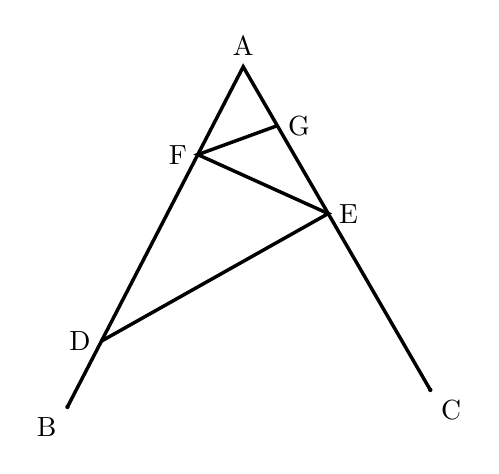
\begin{tikzpicture}[baseline = {(current bounding box.north)},x = 0.9cm,y=0.9cm,line width = 1.25pt, scale=0.8]
			\draw (0,0) -- (3.1,6) -- (6.4,0.3);
			\draw (0.6,1.161) -- (4.6,3.41) -- (2.3,4.45) -- (3.7,4.96);
			\node at (0,0) [below left ]{B};
			\node at (0.6,1.161) [left] {D};
			\node at (2.3,4.45) [left] {F};
			\node at (3.1,6) [above] {A};
			\node at (3.7,4.96) [right] {G};
			\node at (4.6,3.41) [right] {E};
			\node at (6.4,0.3) [below right] {C};
			\fill (6.4,0.3) circle (1pt);
			\fill (0,0) circle (1pt);
		\end{tikzpicture}
	}
\end{exercise}

\begin{exercise} Justifier sur les figures ci-dessous si les droites $(BC)$ et $(PQ)$ sont parallèles ou non.
	
	\begin{minipage}{0.3\columnwidth} 
		\begin{tikzpicture}[scale=0.65]
			\tkzSetUpPoint[size=3, fill=black]
			\tkzfctset{tan style/.style={->,>=latex, color=red, line width=1.2pt}}  
			\tkzInit[xmin=-3,xmax=3,ymin=-3,ymax=3,xstep=0.5, ystep=0.5];
			%\tkzSetUpLine[add=.5 and .5]
			\tkzDefPoints{0/0/B,3.5/0/C, -0.8/0/D, 4.3/0/E}
			\tkzDefTriangle[two angles=52 and 62](B,C)\tkzGetPoint{A}
			\tkzDrawPolygon[line width=1.2pt](A,B,C)
			\tkzDefPointWith[linear,K=0.6](A,B) \tkzGetPoint{P}
			\tkzDefPointWith[linear,K=0.6](A,C) \tkzGetPoint{Q}
			\tkzDefPointWith[linear,K=-0.3](Q,P) \tkzGetPoint{P'}
			\tkzDrawLine[add=0.0 and 0.0 , line width=1.2pt](P,Q)
			\tkzDrawSegment[ line width=1.2pt](B,C)
			\tkzLabelPoints[  font=\scriptsize](C) 
			\tkzLabelPoints[below left, font=\scriptsize](B) 
			\tkzLabelPoints[above, font=\scriptsize](A)
			\tkzLabelPoints[above left, font=\scriptsize](P) 
			\tkzLabelPoints[below  left, font=\scriptsize](Q) 
			\tkzMarkAngle[mark=none,-, >=latex, size =0.7](P,A,Q)
			\tkzLabelAngles[pos=1.3, fill = white ](P,A,Q){\scriptsize$\ang{66}$}
			\tkzMarkAngle[mark=none,-, >=latex, size =0.65](C,B,A)
			\tkzLabelAngles[pos=1.4, fill = white ](C,B,A){\scriptsize$\ang{55}$}
			\tkzMarkAngle[mark=none,-, >=latex, size =0.65](A,Q,P)
			\tkzLabelAngles[pos=1.3, fill = white ](A,Q,P){\scriptsize$\ang{56}$}
			% \tkzDrawSegment[dim={$5$,25pt,}](A,P))
			%  \tkzDrawSegment[dim={$5$,25pt,}](A,P))
		\end{tikzpicture}
	\end{minipage}\hfill
	\begin{minipage}{0.3\columnwidth} 
		\begin{tikzpicture}[scale=0.60]
			\tkzSetUpPoint[size=3, fill=black]
			\tkzfctset{tan style/.style={->,>=latex, color=red, line width=1.2pt}}  
			\tkzInit[xmin=-3,xmax=3,ymin=-3,ymax=3,xstep=0.5, ystep=0.5];
			%\tkzSetUpLine[add=.5 and .5]
			\tkzDefPoints{0/0/B,3.5/0/C, -0.8/0/D, 4.3/0/E}
			\tkzDefTriangle[two angles=52 and 62](B,C)\tkzGetPoint{A}
			\tkzDrawPolygon[line width=1.2pt](A,B,C)
			\tkzDefPointWith[linear,K=0.6](A,B) \tkzGetPoint{P}
			\tkzDefPointWith[linear,K=0.6](A,C) \tkzGetPoint{Q}
			\tkzDefPointWith[linear,K=-0.3](Q,P) \tkzGetPoint{P'}
			\tkzDrawLine[add=0.0 and 0.0 , line width=1.2pt](P,Q)
			\tkzDrawSegment[ line width=1.2pt](B,C)
			\tkzLabelPoints[  font=\scriptsize](C) 
			\tkzLabelPoints[below left, font=\scriptsize](B) 
			\tkzLabelPoints[above, font=\scriptsize](A)
			\tkzLabelPoints[below right, font=\scriptsize](P) 
			\tkzLabelPoints[below  left, font=\scriptsize](Q) 
			%\tkzMarkAngle[mark=none,-, >=latex, size =0.7](P,A,Q)
			%\tkzLabelAngles[pos=1.2, fill = white](P,A,Q){$\ang{68}$}
			%\tkzMarkAngle[mark=none,-, >=latex, size =0.65](C,B,A)
			%\tkzLabelAngles[pos=1.45, fill = white](C,B,A){$\ang{55}$}
			%\tkzMarkAngle[mark=none,-, >=latex, size =0.65](A,Q,P)
			%\tkzLabelAngles[pos=1.25, fill = white](A,Q,P){$\ang{56}$}
			\tkzDrawSegment[dim={\scriptsize$6$,16pt,}](A,Q))
			\tkzDrawSegment[dim={\scriptsize$0.5$,16pt,}](Q,C))
			\tkzDrawSegment[dim={\scriptsize$7.8$,-16pt,}](A,P))
			\tkzDrawSegment[dim={\scriptsize$8.45$,-32pt,}](A,B)
		\end{tikzpicture}
	\end{minipage}\hfill 
	\begin{minipage}{0.3\columnwidth} 
		\begin{tikzpicture}[scale=0.60]
			\tkzSetUpPoint[size=3, fill=black]
			\tkzfctset{tan style/.style={->,>=latex, color=red, line width=1.2pt}}  
			\tkzInit[xmin=-3,xmax=3,ymin=-3,ymax=3,xstep=0.5, ystep=0.5];
			%\tkzSetUpLine[add=.5 and .5]
			\tkzDefPoints{0/0/B,3.2/0/C, -0.8/0/D, 4.3/0/E}
			\tkzDefTriangle[two angles=56 and 68](B,C)\tkzGetPoint{A}
			\tkzDrawPolygon[line width=1.2pt](A,B,C)
			\tkzDefPointWith[linear,K=0.6](A,B) \tkzGetPoint{P}
			\tkzDefPointWith[linear,K=0.6](A,C) \tkzGetPoint{Q}
			\tkzDefPointWith[linear,K=-0.3](Q,P) \tkzGetPoint{P'}
			\tkzDrawLine[add=0.0 and 0.0 , line width=1.2pt](P,Q)
			\tkzDrawSegment[ line width=1.2pt](B,C)
			\tkzLabelPoints[  font=\scriptsize](C) 
			\tkzLabelPoints[below left, font=\scriptsize](B) 
			\tkzLabelPoints[above, font=\scriptsize](A)
			\tkzLabelPoints[above left, font=\scriptsize](P) 
			\tkzLabelPoints[below  left, font=\scriptsize](Q) 
			\tkzMarkAngle[mark=none,-, >=latex, size =0.7](P,A,Q)
			%\tkzLabelAngles[pos=1.3, fill = white](P,A,Q){$\ang{68}$}
			\tkzMarkAngle[mark=none,-, >=latex, size =0.65](C,B,A)
			\tkzLabelAngles[pos=1.5, fill = white ](C,B,A){\scriptsize$\ang{56}$}
			\tkzMarkAngle[mark=none,-, >=latex, size =0.65](A,Q,P)
			\tkzLabelAngles[pos=1.3, fill = white ](A,Q,P){\scriptsize$\ang{68}$} 
			% \tkzDrawSegment[dim={$5$,25pt,}](A,P))
			%  \tkzDrawSegment[dim={$5$,25pt,}](A,P))
			\tkzMarkSegments[mark=s||](A,Q Q,P)
		\end{tikzpicture}
	\end{minipage}
	\\
	\begin{minipage}{0.3\columnwidth} \centering
		\begin{tikzpicture}[baseline={(E)},scale=0.90]
			\tkzDefPoint(0,0){A} 
			\tkzDefPoint(2.7 ,2){E}
			\tkzDefPoint(3.5,-1.3){D}
			\tkzDefPointsBy[homothety = center A ratio 0.7](D){C}
			\tkzDefPointsBy[homothety = center A ratio 0.7](E){B} 
			\tkzDrawSegments[line width=1.2pt](A,E A,D B,C E,D)
			\tkzSetUpPoint[size=2, fill=black]
			\tkzDrawPoints(A,B,C,D,E)
			\tkzLabelPoint[below left](C){\scriptsize $C$}	
			\tkzLabelPoint[ left, font=\scriptsize](A){\scriptsize $A$}		
			\tkzLabelPoint[above left, font=\scriptsize](B){\scriptsize $B$}		
			\tkzLabelPoint[above right, font=\scriptsize](E){\scriptsize $E$}		
			\tkzLabelPoint[below right, font=\scriptsize](D){\scriptsize $D$}
			\tkzLabelSegment[above,sloped ](B,A){\scriptsize $3.12$}	
			\tkzDrawSegment[dim={\scriptsize$5$,16pt,}](A,E)		
			\tkzLabelSegment[above right](C,A){\scriptsize $4$}	 
			\tkzDrawSegment[dim={\scriptsize$6.4$,-16pt,}](A,D)		
		\end{tikzpicture} 
	\end{minipage} 
	\hfill
	\begin{minipage}{0.3\columnwidth} 
		\begin{tikzpicture}[scale=1.0] 
			\tkzSetUpPoint[size=3, fill=black]
			\tkzfctset{tan style/.style={->,>=latex, color=red, line width=1.2pt}}   
			\tkzSetUpLine[line width= 1.2pt, add=.5 and .5] 	
			\def \a{1.6}; 
			\def \b{2.0}; 
			\tkzDefPoint(0,0){A}
			\tkzDefShiftPoint[A](-15:\a){B}
			\tkzDefShiftPoint[A](20:\b){C}
			\tkzDefPointBy[homothety=center A ratio -1.5 ](B)\tkzGetPoint{P}
			\tkzDefPointBy[homothety=center A ratio -1.5 ](C)\tkzGetPoint{Q} 
			\tkzDrawPolygon[line width=1.2pt](A,B,C)
			\tkzDrawPolygon[line width=1.2pt](A,P,Q)
			\tkzLabelSegment[font=\scriptsize, sloped, below](A,B){$\SI{1.7}{\centi\meter}$}
			\tkzLabelSegment[font=\scriptsize, sloped, above](A,C){$\SI{1.3}{\centi\meter}$}
			%	\tkzLabelSegment[font=\scriptsize, sloped, below](B,C){$\SI{3.4}{\centi\meter}$}
			\tkzLabelSegment[font=\scriptsize, sloped, above](A,P){$\SI{2.6}{\centi\meter}$}
			\tkzLabelSegment[font=\scriptsize, sloped, below](A,Q){$\SI{3.4}{\centi\meter}$}
			%	\tkzLabelSegment[font=\scriptsize, sloped, above](P,Q){$y$}
			\tkzLabelPoints[font=\scriptsize, left](Q)
			\tkzLabelPoints[font=\scriptsize, below right](B)
			\tkzLabelPoints[font=\scriptsize, above right](C)
			\tkzLabelPoints[font=\scriptsize, above left](A,P) 
		\end{tikzpicture}  
	\end{minipage} 
	\hfill
	\begin{minipage}{0.3\columnwidth} 
		\begin{tikzpicture}[scale=0.60]
			\tkzSetUpPoint[size=3, fill=black]
			\tkzfctset{tan style/.style={->,>=latex, color=red, line width=1.2pt}}  
			\tkzInit[xmin=-3,xmax=3,ymin=-3,ymax=3,xstep=0.5, ystep=0.5];
			%\tkzSetUpLine[add=.5 and .5]
			\tkzDefPoints{0/0/B,3.5/0/C, -0.8/0/D, 4.3/0/E}
			\tkzDefTriangle[two angles=90 and 36](B,C)\tkzGetPoint{A}
			\tkzDrawPolygon[line width=1.2pt](A,B,C)
			\tkzDefPointWith[linear,K=0.4](A,B) \tkzGetPoint{P}
			\tkzDefPointWith[linear,K=0.4](A,C) \tkzGetPoint{Q}
			\tkzDefPointWith[linear,K=-0.3](Q,P) \tkzGetPoint{P'}
			\tkzDrawLine[add=0.0 and 0.0 , line width=1.2pt](P,Q)
			\tkzDrawSegment[ line width=1.2pt](B,C)
			\tkzLabelPoints[  font=\scriptsize](C) 
			\tkzLabelPoints[below left, font=\scriptsize](B) 
			\tkzLabelPoints[above, font=\scriptsize](A)
			\tkzLabelPoints[below right, font=\scriptsize](P) 
			\tkzLabelPoints[below  left, font=\scriptsize](Q) 
			%\tkzMarkAngle[mark=none,-, >=latex, size =0.7](P,A,Q)
			%\tkzLabelAngles[pos=1.2, fill = white](P,A,Q){$\ang{68}$}
			%\tkzMarkAngle[mark=none,-, >=latex, size =0.65](C,B,A)
			%\tkzLabelAngles[pos=1.45, fill = white](C,B,A){$\ang{55}$}
			%\tkzMarkAngle[mark=none,-, >=latex, size =0.65](A,Q,P)
			%\tkzLabelAngles[pos=1.25, fill = white](A,Q,P){$\ang{56}$}
			%\tkzDrawSegment[dim={$5$,25pt,}](A,Q))
			\tkzMarkRightAngle(Q,P,A)
			\tkzLabelSegment[below](P,Q){\scriptsize$4$}
			\tkzDrawSegment[dim={$10.5$,25pt,}](Q,C))
			\tkzDrawSegment[dim={$3$,-16pt,}](A,P))
			\tkzDrawSegment[dim={$6.3$,-16pt,}](P,B)
		\end{tikzpicture}
	\end{minipage}\\
	\begin{minipage}{0.23\columnwidth} 
		\begin{tikzpicture}[scale=1.0] 
			\tkzSetUpPoint[size=3, fill=black]
			\tkzfctset{tan style/.style={->,>=latex, color=red, line width=1.2pt}}   
			\tkzSetUpLine[line width= 1.2pt, add=.5 and .5] 	
			\def \a{1.3}; 
			\def \b{1.9}; 
			\tkzDefPoint(0,0){A}
			\tkzDefShiftPoint[A](-110:\a){B}
			\tkzDefShiftPoint[A](-40:\b){C}
			\tkzDefPointBy[homothety=center A ratio -1.3 ](B)\tkzGetPoint{P}
			\tkzDefPointBy[homothety=center A ratio -1.3 ](C)\tkzGetPoint{Q} 
			\tkzDrawPolygon[line width=1.2pt](A,B,C)
			\tkzDrawPolygon[line width=1.2pt](A,P,Q)
			\tkzLabelSegment[font=\scriptsize, sloped, above](A,B){$\SI{1.8}{\meter}$}
			\tkzLabelSegment[font=\scriptsize, sloped, above](A,C){$\SI{2.7}{\meter}$}
			%	\tkzLabelSegment[font=\scriptsize, sloped, below](B,C){$\SI{3.4}{\centi\meter}$}
			\tkzLabelSegment[font=\scriptsize, sloped, below](A,P){$\SI{5}{\meter}$}
			\tkzLabelSegment[font=\scriptsize, sloped, below](A,Q){$\SI{7.6}{\meter}$}
			%	\tkzLabelSegment[font=\scriptsize, sloped, above](P,Q){$y$}
			\tkzLabelPoints[font=\scriptsize, left](Q)
			\tkzLabelPoints[font=\scriptsize, below right](B)
			\tkzLabelPoints[font=\scriptsize, above right](C)
			\tkzLabelPoints[font=\scriptsize, right](A,P) 
		\end{tikzpicture}  
	\end{minipage} 
	\hfill 
	\begin{minipage}{0.23\columnwidth} 
		\begin{tikzpicture}[scale=1.0] 
			\tkzSetUpPoint[size=3, fill=black]
			\tkzfctset{tan style/.style={->,>=latex, color=red, line width=1.2pt}}   
			\tkzSetUpLine[line width= 1.2pt, add=.5 and .5] 	
			\def \a{1.3}; 
			\def \b{1.9}; 
			\tkzDefPoint(0,0){A}
			\tkzDefShiftPoint[A](-110:\a){B}
			\tkzDefShiftPoint[A](-40:\b){C}
			\tkzDefPointBy[homothety=center A ratio -1.3 ](B)\tkzGetPoint{P}
			\tkzDefPointBy[homothety=center A ratio -1.3 ](C)\tkzGetPoint{Q} 
			\tkzDrawPolygon[line width=1.2pt](A,B,C)
			\tkzDrawPolygon[line width=1.2pt](A,P,Q)
			\tkzLabelSegment[font=\scriptsize, sloped, above](A,B){$\SI{42}{\centi\meter}$}
			\tkzLabelSegment[font=\scriptsize, sloped, above](A,C){$\SI{32.4}{\centi\meter}$}
			%	\tkzLabelSegment[font=\scriptsize, sloped, below](B,C){$\SI{3.4}{\centi\meter}$}
			\tkzLabelSegment[font=\scriptsize, sloped, below](A,P){$\SI{70}{\centi\meter}$}
			\tkzLabelSegment[font=\scriptsize, sloped, below](A,Q){$\SI{54}{\centi\meter}$}
			%	\tkzLabelSegment[font=\scriptsize, sloped, above](P,Q){$y$}
			\tkzLabelPoints[font=\scriptsize, left](Q)
			\tkzLabelPoints[font=\scriptsize, below right](B)
			\tkzLabelPoints[font=\scriptsize, above right](C)
			\tkzLabelPoints[font=\scriptsize, right](A,P) 
		\end{tikzpicture}  
	\end{minipage} 
	\hfill 
	\begin{minipage}{0.23\columnwidth} 
		\begin{tikzpicture}[scale=1.0] 
			\tkzSetUpPoint[size=3, fill=black]
			\tkzfctset{tan style/.style={->,>=latex, color=red, line width=1.2pt}}   
			\tkzSetUpLine[line width= 1.2pt, add=.5 and .5] 	
			\def \a{1.3}; 
			\def \b{1.9}; 
			\tkzDefPoint(0,0){A}
			\tkzDefShiftPoint[A](-110:\a){B}
			\tkzDefShiftPoint[A](-40:\b){C}
			\tkzDefPointBy[homothety=center A ratio -1.3 ](B)\tkzGetPoint{P}
			\tkzDefPointBy[homothety=center A ratio -1.3 ](C)\tkzGetPoint{Q} 
			\tkzDrawPolygon[line width=1.2pt](A,B,C)
			\tkzDrawPolygon[line width=1.2pt](A,P,Q)
			\tkzLabelSegment[font=\scriptsize, sloped, above](A,B){$\SI{45}{\centi\meter}$}
			%		\tkzLabelSegment[font=\scriptsize, sloped, above](A,C){$\SI{32.4}{\centi\meter}$}
			\tkzLabelSegment[font=\scriptsize, sloped, below](B,C){$\SI{76}{\centi\meter}$}
			\tkzLabelSegment[font=\scriptsize, sloped, below](A,P){$\SI{60}{\centi\meter}$}
			%		\tkzLabelSegment[font=\scriptsize, sloped, below](A,Q){$\SI{54}{\centi\meter}$}
			\tkzLabelSegment[font=\scriptsize, sloped, above](P,Q){$\SI{100}{\centi\meter}$}
			\tkzLabelPoints[font=\scriptsize, left](Q)
			\tkzLabelPoints[font=\scriptsize, below right](B)
			\tkzLabelPoints[font=\scriptsize, above right](C)
			\tkzLabelPoints[font=\scriptsize, right](A,P) 
		\end{tikzpicture}  
	\end{minipage} 
	\hfill 
	\begin{minipage}{0.23\columnwidth} 
		\begin{tikzpicture}[scale=1.0] 
			\tkzSetUpPoint[size=3, fill=black]
			\tkzfctset{tan style/.style={->,>=latex, color=red, line width=1.2pt}}   
			\tkzSetUpLine[line width= 1.2pt, add=.5 and .5] 	
			\def \a{1.3}; 
			\def \b{1.9}; 
			\tkzDefPoint(0,0){A}
			\tkzDefShiftPoint[A](-110:\a){B}
			\tkzDefShiftPoint[A](-40:\b){C}
			\tkzDefPointBy[homothety=center A ratio -1.3 ](B)\tkzGetPoint{P}
			\tkzDefPointBy[homothety=center A ratio -1.3 ](C)\tkzGetPoint{Q} 
			\tkzDrawPolygon[line width=1.2pt](A,B,C)
			\tkzDrawPolygon[line width=1.2pt](A,P,Q)
			\tkzLabelSegment[font=\scriptsize, sloped, above](A,B){$\SI{2.4}{\centi\meter}$}
			%		\tkzLabelSegment[font=\scriptsize, sloped, above](A,C){$\SI{32.4}{\centi\meter}$}
			\tkzLabelSegment[font=\scriptsize, sloped, below](B,C){$\SI{4.3}{\centi\meter}$}
			\tkzLabelSegment[font=\scriptsize, sloped, below](A,P){$\SI{3.3}{\centi\meter}$}
			%		\tkzLabelSegment[font=\scriptsize, sloped, below](A,Q){$\SI{54}{\centi\meter}$}
			\tkzLabelSegment[font=\scriptsize, sloped, above](P,Q){$\SI{5.9}{\centi\meter}$}
			\tkzLabelPoints[font=\scriptsize, left](Q)
			\tkzLabelPoints[font=\scriptsize, below right](B)
			\tkzLabelPoints[font=\scriptsize, above right](C)
			\tkzLabelPoints[font=\scriptsize, right](A,P) 
		\end{tikzpicture}  
	\end{minipage} 
\end{exercise}%

\begin{exercise}[Métropole 2017] \hfill  
	
	Pour illustrer l'exercice, la figure ci-dessous a été faite à main levée.
	
	Les points $D$, $F$, $A$ et $B$ sont alignés, ainsi que les points $E$, $G$, $A$ et $C$. De plus, les droites $(DE)$ et $(FG)$ sont parallèles.
	
	\begin{minipage}{1\columnwidth}\centering 
		\begin{tikzpicture} [scale=0.4]
			\tkzSetUpPoint[size=2, fill=black]
			\tkzfctset{tan style/.style={->,>=latex, color=red, line width=1.2pt}}   
			\tkzSetUpLine[line width= 1.2pt, add=.5 and .5] 
			\tkzDefPoint(0,0){A}
			\tkzDefShiftPoint[A](220:4){G}
			\tkzDefShiftPoint[A](40:5){C}
			\tkzDefShiftPoint[A](220:10.8){E}
			\tkzInterCC[R](A,5 cm)(G,3 cm) \tkzGetSecondPoint{F}
			\tkzDefPointWith[linear, K=-1.25](A,F) \tkzGetPoint{B}
			\tkzDefLine[parallel = through E](F,G)
			\tkzInterLL(A,F)(E,tkzPointResult) \tkzGetPoint{D} 
			\tkzDrawSegments[decorate, decoration={snake, amplitude=.3mm}](A,B B,C C,A A,F A,G F,G G,E F,D  D,E)
			
			\pgfresetboundingbox % removes white space
			
			\tkzSetUpPoint[size=5, fill=black] 
			% 			\tkzDrawPoints(A,B,C,D,E,F,G)  
			\tkzLabelPoints[right,font=\scriptsize](B)
			\tkzLabelPoints[above,font=\scriptsize](C,F)
			\tkzLabelPoints[left,font=\scriptsize](D)
			\tkzLabelPoints[below,font=\scriptsize](E)
			\tkzLabelPoints[below right,font=\scriptsize](G)
			\tkzLabelPoints[above left,font=\scriptsize](A)
			\tkzLabelSegment[midway, sloped, below,font=\scriptsize](E,D){ 8,1 \si{\centi\meter}};
			\tkzLabelSegment[midway, sloped, below,font=\scriptsize](E,G){ 6,8 \si{\centi\meter}};
			\tkzLabelSegment[midway, sloped, below,font=\scriptsize](G,A){ 4 \si{\centi\meter}};
			\tkzLabelSegment[midway, sloped, above,font=\scriptsize](F,A){ 5 \si{\centi\meter}};
			\tkzLabelSegment[midway, sloped, above,font=\scriptsize](A,C){ 5 \si{\centi\meter}};
			\tkzLabelSegment[midway, sloped, below,font=\scriptsize](A,B){ 6,25 \si{\centi\meter}};
		\end{tikzpicture}
	\end{minipage}
	
	
	\begin{enumerate}[label=\alph*),leftmargin=*]
		\item Montrer que le triangle $AFG$ est un triangle rectangle.
		\item Calculer la longueur du segment $[AD]$. En déduire la longueur du segment $[FD]$.
		\item Les droites $(FG)$ et $(BC)$ sont-elles parallèles ? Justifier.
	\end{enumerate} 
\end{exercise} 


%----------------------------------------------------------------------------------------
%	EXERCICES
%----------------------------------------------------------------------------------------

\newpage 

\begin{exercise}[Brevet 2018] 
	Avec un logiciel de géométrie dynamique, on a construit la figure A.
	En appliquant à la figure A des homothéties de centre O et de rapports différents, on a
	ensuite obtenu les autres figures. 
	\begin{figure}[h]
		\begin{tikzpicture} [scale=0.5] 
			\tkzSetUpPoint[size=5, fill=black]
			\tkzDefPoint(2,1.8){A0}
			\tkzDefPoint(3.8,0.4){A1}
			\tkzDefPoint(3.2,0.7){A2}
			\tkzDefPoint(2.4,1){A3}
			\tkzDefPoint(0,0){O}
			\tkzDefPoint(10.5,9.45){U}
			\tkzDefPoint(19.5,2.1){V}
			\tkzDrawPolygon[line width=1.2pt, fill = gray!20](A0,A1,A2,A3)
			\foreach \i in {2,3,4,5}{%
				\foreach \j in {0,1,2,3}{
					\tkzDefPointsBy[homothety = center O ratio \i](A\j){A\i\j}
				}
				\tkzDrawPolygon[line width=1.2pt, fill = gray!20 ](A\i0,A\i1,A\i2,A\i3)
			}
			\tkzDrawLine[add=0 and 0](O,U)
			\tkzDrawLine[add=0 and 0](O,V) 
			\tkzDrawPoints(O,A0,  A20, A30, A40, A50) 
			\tkzLabelPoint[below left](O){$O$} 
			\tkzLabelPoint[above left](A0){$A$} 
			\tkzLabelPoint[above left](A20){$B$} 
			\tkzLabelPoint[above left](A30){$C$} 
			\tkzLabelPoint[above left](A40){$D$} 
			\tkzLabelPoint[above left](A50){$E$} 
			\tkzMarkSegments[mark=s||](O,A0 A0,A20 A20,A30 A30,A40 A40,A50);
			\tkzText(2.6,1.3){\scriptsize Figure A}
			\tkzText(5.2,2.6){\scriptsize Figure B}
			\tkzText(7.8,3.9){\scriptsize Figure C}
			\tkzText(10.4,5.2){\scriptsize Figure D}
			\tkzText(13,6.5){\scriptsize Figure E}
		\end{tikzpicture} 
	\end{figure} 
	\begin{enumerate}[label=\alph*),leftmargin=*]
		\item   Quel est le rapport de l'homothétie de centre $O$ qui permet d'obtenir la figure $C$ à
		partir de la figure $A$ ? \emph{Aucune justification n'est attendue.}
		\item   On applique l'homothétie de centre $O$ et de rapport $\frac{3}{5}$ à la figure E. Quelle figure obtient-on ? \emph{Aucune justification n'est attendue.}
		\item   Quelle figure a une aire quatre fois plus grande que celle de la figure A ? Justifier.
	\end{enumerate} 
\end{exercise} 

\begin{exercise}  
	Les deux rectangles A et B sont semblables. 
	\begin{figure}[h]
		\begin{tikzpicture}
			\tkzDefPoint(-2,-1.5){A}
			\tkzDefPoint(2.5,-1.5){B}
			\tkzDefPoint(2.5,1){C}
			\tkzDefPoint(-2,1){D}
			\tkzDrawSegments[line width=1.2pt](A,B B,C C,D D,A)
			\tkzLabelSegment[below](A,B){$\numprint{6}\si{\centi\meter}$}
			%		\tkzLabelSegment[right](B,C){$\numprint{6}\si{\centi\meter}$}
			%		\tkzMarkRightAngle[  size=0.25](B,A,D) 
			%		\tkzMarkRightAngle[  size=0.25](C,B,A) 
			%		\tkzMarkRightAngle[  size=0.25](D,C,B) 
			%		\tkzMarkRightAngle[  size=0.25](A,D,C) 
			\tkzLabelSegment[below](A,C){$B$}
			\begin{scope}[ shift={(-6,0)} , scale=0.63]
				\tkzDefPoint(-2,-1.5){A}
				\tkzDefPoint(2.5,-1.5){B}
				\tkzDefPoint(2.5,1){C}
				\tkzDefPoint(-2,1){D}
				\tkzDrawSegments[line width=1.2pt](A,B B,C C,D D,A)
				\tkzLabelSegment[below](A,B){$\numprint{2.5}\si{\centi\meter}$}
				\tkzLabelSegment[right](B,C){$\numprint{4}\si{\centi\meter}$}
				%			\tkzMarkRightAngle[  size=0.25](B,A,D) 
				%			\tkzMarkRightAngle[  size=0.25](C,B,A) 
				%			\tkzMarkRightAngle[  size=0.25](D,C,B) 
				%			\tkzMarkRightAngle[  size=0.25](A,D,C) 
				\tkzLabelSegment[below](A,C){$A$}
			\end{scope}
		\end{tikzpicture}  
	\end{figure} 
	\begin{enumerate}[label=\alph*),leftmargin=*]
		\item Calculer l'aire du rectangle $B$. 
		\item Quel rapport d'agrandissement du rectangle $A$ donne le rectangle $B$ ?
	\end{enumerate}
\end{exercise}
\begin{exercise}  
	Les deux rectangles A et B sont semblables. 
	\begin{figure}[h]
		\begin{tikzpicture}
			\tkzDefPoint(-2,-1.5){A}
			\tkzDefPoint(2.5,-1.5){B}
			\tkzDefPoint(2.5,1){C}
			\tkzDefPoint(-2,1){D}
			\tkzDrawSegments[line width=1.2pt](A,B B,C C,D D,A)
			\tkzLabelSegment[below](A,B){$\numprint{6.25}\si{\centi\meter}$}
			\tkzLabelSegment[right](B,C){$\numprint{3}\si{\centi\meter}$}
			%		\tkzMarkRightAngle[  size=0.25](B,A,D) 
			%		\tkzMarkRightAngle[  size=0.25](C,B,A) 
			%		\tkzMarkRightAngle[  size=0.25](D,C,B) 
			%		\tkzMarkRightAngle[  size=0.25](A,D,C) 
			\tkzLabelSegment[below](A,C){$B$}
			\begin{scope}[ shift={(-6,0)} , scale=0.63]
				\tkzDefPoint(-2,-1.5){A}
				\tkzDefPoint(2.5,-1.5){B}
				\tkzDefPoint(2.5,1){C}
				\tkzDefPoint(-2,1){D}
				\tkzDrawSegments[line width=1.2pt](A,B B,C C,D D,A)
				%				\tkzLabelSegment[below](A,B){$\numprint{2}\si{\centi\meter}$}
				\tkzLabelSegment[right](B,C){$\numprint{2}\si{\centi\meter}$}
				%			\tkzMarkRightAngle[  size=0.25](B,A,D) 
				%			\tkzMarkRightAngle[  size=0.25](C,B,A) 
				%			\tkzMarkRightAngle[  size=0.25](D,C,B) 
				%			\tkzMarkRightAngle[  size=0.25](A,D,C) 
				\tkzLabelSegment[below](A,C){$A$}
			\end{scope}
		\end{tikzpicture}  
	\end{figure} 
	\begin{enumerate}[label=\alph*),leftmargin=*]
		\item Calculer l'aire du rectangle $B$. 
		\item Quel rapport de réduction du rectangle $B$ donne le rectangle $A$ ?
	\end{enumerate} 
\end{exercise}

\begin{exercise}  
	Les deux rectangles A et B sont semblables.  
	\begin{figure}[h]
		\begin{tikzpicture}
			\tkzDefPoint(-2,-1.5){A}
			\tkzDefPoint(2.5,-1.5){B}
			\tkzDefPoint(2.5,1){C}
			\tkzDefPoint(-2,1){D}
			\tkzDrawSegments[line width=1.2pt](A,B B,C C,D D,A)
			%			\tkzLabelSegment[below](A,B){$3x$}
			\tkzLabelSegment[right](B,C){$3x$}
			%		\tkzMarkRightAngle[  size=0.25](B,A,D) 
			%		\tkzMarkRightAngle[  size=0.25](C,B,A) 
			%		\tkzMarkRightAngle[  size=0.25](D,C,B) 
			%		\tkzMarkRightAngle[  size=0.25](A,D,C) 
			\tkzLabelSegment[below](A,C){$B$}
			\begin{scope}[ shift={(-6,0)} , scale=0.63]
				\tkzDefPoint(-2,-1.5){A}
				\tkzDefPoint(2.5,-1.5){B}
				\tkzDefPoint(2.5,1){C}
				\tkzDefPoint(-2,1){D}
				\tkzDrawSegments[line width=1.2pt](A,B B,C C,D D,A)
				\tkzLabelSegment[below](A,B){$x+2$}
				\tkzLabelSegment[right](B,C){$x$}
				%			\tkzMarkRightAngle[  size=0.25](B,A,D) 
				%			\tkzMarkRightAngle[  size=0.25](C,B,A) 
				%			\tkzMarkRightAngle[  size=0.25](D,C,B) 
				%			\tkzMarkRightAngle[  size=0.25](A,D,C) 
				\tkzLabelSegment[below](A,C){$A$}
			\end{scope}
		\end{tikzpicture}  
	\end{figure} 
	L'aire du rectangle B est \SI{35}{\centi\meter^2}. Calculer l'aire du rectangle $A$.
\end{exercise}

\begin{exercise}  
	Les deux rectangles A et B sont semblables. 
	\begin{figure}[h]
		\begin{tikzpicture}
			\tkzDefPoint(-2,-1.5){A}
			\tkzDefPoint(2.5,-1.5){B}
			\tkzDefPoint(2.5,1){C}
			\tkzDefPoint(-2,1){D}
			\tkzDrawSegments[line width=1.2pt](A,B B,C C,D D,A)
			%			\tkzLabelSegment[below](A,B){$3x$}
			%		\tkzLabelSegment[right](B,C){$3x$}
			%		\tkzMarkRightAngle[  size=0.25](B,A,D) 
			%		\tkzMarkRightAngle[  size=0.25](C,B,A) 
			%		\tkzMarkRightAngle[  size=0.25](D,C,B) 
			%		\tkzMarkRightAngle[  size=0.25](A,D,C) 
			\tkzLabelSegment[below](A,C){$B$}
			\begin{scope}[ shift={(-6,0)} , scale=0.63]
				\tkzDefPoint(-2,-1.5){A}
				\tkzDefPoint(2.5,-1.5){B}
				\tkzDefPoint(2.5,1){C}
				\tkzDefPoint(-2,1){D}
				\tkzDrawSegments[line width=1.2pt](A,B B,C C,D D,A)
				\tkzLabelSegment[below](A,B){$6~\si{\centi\meter}$}
				\tkzLabelSegment[right](B,C){$2~\si{\centi\meter}$}
				%			\tkzMarkRightAngle[  size=0.25](B,A,D) 
				%			\tkzMarkRightAngle[  size=0.25](C,B,A) 
				%			\tkzMarkRightAngle[  size=0.25](D,C,B) 
				%			\tkzMarkRightAngle[  size=0.25](A,D,C) 
				\tkzLabelSegment[below](A,C){$A$}
			\end{scope}
		\end{tikzpicture}   
	\end{figure} 
	L'aire du rectangle B est \SI{35}{\centi\meter^2}. Calculer son périmètre. 
\end{exercise} 

\begin{exercise}[d'après une question vue au Brevet] 
	Mon rectangle est semblable à un rectangle de côtés $3$\si{\centi\meter} et $2$\si{\centi\meter}. Sont aire est \SI{37.5}{\centi\meter^2}. Quel est son périmètre ?
\end{exercise}
%----------------------------------------------------------------------------------------
% 
%----------------------------------------------------------------------------------------

\newpage 
\loadgeometry{widelayout}  
\pagestyle{scrheadings} % Print headers again  
\KOMAoptions{
	headwidth=textwithmarginpar,
	headsepline=true,
	headsepline= 0.5pt,
	footwidth=textwithmarginpar,
} 
\onehalfspacing  
\section{Critères de similitude des triangles}

\begin{postulat}[Critère de similitude CCC] Si les longueurs des 3 côtés d'un triangle $T_1$ sont \textbf{proportionnelles} aux longueurs respectives des 3 côtés d'un triangle $T_2$, alors les deux triangles sont semblables.
\end{postulat}
\begin{postulat}[Critère de similitude AA] Si 2 angles d'un triangle $T_1$ sont \textbf{respectivement égaux} à 2 angles d'un triangle $T_2$. Alors les deux triangles sont semblables.  
\end{postulat}

\begin{postulat}[Critère CAC-Semblable] Si deux triangles $T_1$ et $T_2$ ont un angle égal compris entre 2 côtés respectivement proportionnels, alors les deux triangles sont semblables.  
\end{postulat}
%On passe de l'un à l'autre par un \emph{agrandissement} ou une \emph{réduction}.

%----------------------------------------------------------------------------------------
%	EXERCICES
%----------------------------------------------------------------------------------------

%\newpage 
%\loadgeometry{widelayout}  
%\pagestyle{scrheadings} % Print headers again  
%\KOMAoptions{
%	headwidth=textwithmarginpar,
%	headsepline=true,
%	headsepline= 0.5pt,
%	footwidth=textwithmarginpar,
%} 
%\onehalfspacing
\subsection{Exercices}

\begin{example}[Triangles semblables]\hfill 
	
	Si possible, démontrer que les paires de triangles sont semblables. 
	\begin{enumerate}[label=\alph*),leftmargin=*]
		\item Préciser les angles de même mesure et les angles correspondants.
		\item Écrire les rapports égaux.
		\item Donner alors un rapport de réduction, et d'agrandissement.
		\item Calculer les longueurs manquantes.
	\end{enumerate} 
	
	\noindent 
	\parbox[position=t]{0.45\textwidth}{
		%\begin{figure}[A]\centering
		\begin{tikzpicture}[scale=1.0]
			\tkzText(0.5,2.8){$(A)$}
			\tkzSetUpPoint[size=3, fill=black]
			\tkzfctset{tan style/.style={->,>=latex, color=red, line width=1.2pt}}   
			\tkzSetUpLine[line width= 1.2pt, add=.5 and .5] 
			\tkzDefPoint(0.0,0){A} 
			\tkzDefShiftPoint[A](0:3.5){B}
			\tkzDefTriangle[two angles=65 and 35](A,B)\tkzGetPoint{C}  
			\tkzDrawPolygon[line width=1.2pt](A,B,C)
			\tkzLabelPoints[above,font=\scriptsize](C)
			\tkzLabelPoints[right,font=\scriptsize](B)
			\tkzLabelPoints[left,font=\scriptsize](A)
			%	\tkzMarkRightAngle[](B,A,C)
			\tkzMarkAngle[mark=none,-, >=latex, size =0.5](B,A,C)
			\tkzMarkAngle[mark=none,-, >=latex, size =0.5](C,B,A)
			\tkzMarkAngle[mark=none,-, >=latex, size =0.5](A,C,B)
			\tkzLabelAngle[font=\scriptsize,pos=.8](B,A,C){$\ang{70}$}
			\tkzLabelAngle[font=\scriptsize,pos=.8](C,B,A){$\ang{30}$}
			\tkzLabelAngle[font=\scriptsize,pos=.8](A,C,B){$\ang{80}$}
			%	\tkzLabelSegment[above, sloped , font=\scriptsize](A,C){\SI{4}{\centi\meter}} 
			\tkzLabelSegment[below, sloped , font=\scriptsize](A,B){\SI{3}{\centi\meter}}
			\tkzLabelSegment[above,sloped ,  font=\scriptsize](C,B){\SI{2}{\centi\meter}}
			\begin{scope}[xshift=4.1cm,yshift=-2cm)] 
				\tkzDefPoint(0.0,0){D} 
				\tkzDefShiftPoint[D](0:5.0){E}
				\tkzDefTriangle[two angles=65 and 40](D,E)\tkzGetPoint{F}  
				\tkzDrawPolygon[line width=1.2pt](D,E,F)
				\tkzLabelPoints[below left,font=\scriptsize](D)
				\tkzLabelPoints[below right,font=\scriptsize](E)
				\tkzLabelPoints[above,font=\scriptsize](F)
				\tkzMarkAngle[mark=none,-, >=latex, size =0.5](E,D,F)
				\tkzMarkAngle[mark=none,-, >=latex, size =0.5](F,E,D)
				\tkzMarkAngle[mark=none,-, >=latex, size =0.5](D,F,E)
				\tkzLabelAngle[font=\scriptsize,pos=.8](E,D,F){$\ang{70}$}
				\tkzLabelAngle[font=\scriptsize,pos=.8](F,E,D){$\ang{30}$}
				\tkzLabelAngle[font=\scriptsize,pos=.8](D,F,E){$\ang{80}$}
				\tkzLabelSegment[below,sloped , font=\scriptsize](D,E){\SI{6}{\centi\meter}}
				%		\tkzLabelSegment[above,sloped , font=\scriptsize](F,E){\SI{6}{\centi\meter}}
				\tkzLabelSegment[above,sloped , font=\scriptsize](D,F){\SI{3}{\centi\meter}}
			\end{scope}
		\end{tikzpicture}   
	} 
	
	\noindent\parbox[position=t]{0.45\textwidth}{
		%\begin{figure}[A]\centering
		\begin{tikzpicture}[scale=1.0]
			\tkzText(0.5,2.8){à vous}
			\tkzSetUpPoint[size=3, fill=black]
			\tkzfctset{tan style/.style={->,>=latex, color=red, line width=1.2pt}}   
			\tkzSetUpLine[line width= 1.2pt, add=.5 and .5] 
			\tkzDefPoint(0.0,0){A} 
			\tkzDefShiftPoint[A](0:3.5){B}
			\tkzDefTriangle[two angles=65 and 35](A,B)\tkzGetPoint{C}  
			\tkzDrawPolygon[line width=1.2pt](A,B,C)
			\tkzLabelPoints[above,font=\scriptsize](C)
			\tkzLabelPoints[right,font=\scriptsize](B)
			\tkzLabelPoints[left,font=\scriptsize](A)
			%	\tkzMarkRightAngle[](B,A,C)
			\tkzMarkAngle[mark=none,-, >=latex, size =0.5](B,A,C)
			\tkzMarkAngle[mark=none,-, >=latex, size =0.5](C,B,A)
			\tkzMarkAngle[mark=none,-, >=latex, size =0.5](A,C,B)
			\tkzLabelAngle[font=\scriptsize,pos=.8](B,A,C){$\ang{70}$}
			\tkzLabelAngle[font=\scriptsize,pos=.8](C,B,A){$\ang{20}$}
			\tkzLabelAngle[font=\scriptsize,pos=.8](A,C,B){$\ang{90}$}
			%	\tkzLabelSegment[above, sloped , font=\scriptsize](A,C){\SI{4}{\centi\meter}} 
			\tkzLabelSegment[below, sloped , font=\scriptsize](A,B){\SI{3}{\centi\meter}}
			\tkzLabelSegment[above,sloped ,  font=\scriptsize](C,B){\SI{4}{\centi\meter}}
			\begin{scope}[xshift=4.8cm,yshift=-0cm)] 
				\tkzDefPoint(0.0,0){D} 
				\tkzDefShiftPoint[D](-20:5.0){E}
				\tkzDefTriangle[two angles=65 and 40](D,E)\tkzGetPoint{F}  
				\tkzDrawPolygon[line width=1.2pt](D,E,F)
				\tkzLabelPoints[below left,font=\scriptsize](D)
				\tkzLabelPoints[below right,font=\scriptsize](E)
				\tkzLabelPoints[above,font=\scriptsize](F)
				\tkzMarkAngle[mark=none,-, >=latex, size =0.5](E,D,F)
				\tkzMarkAngle[mark=none,-, >=latex, size =0.5](F,E,D)
				\tkzMarkAngle[mark=none,-, >=latex, size =0.5](D,F,E)
				\tkzLabelAngle[font=\scriptsize,pos=.8](E,D,F){$\ang{70}$}
				\tkzLabelAngle[font=\scriptsize,pos=.8](F,E,D){$\ang{20}$}
				\tkzLabelAngle[font=\scriptsize,pos=.8](D,F,E){$\ang{90}$}
				\tkzLabelSegment[below,sloped , font=\scriptsize](D,E){\SI{9}{\centi\meter}}
				%		\tkzLabelSegment[above,sloped , font=\scriptsize](F,E){\SI{6}{\centi\meter}}
				\tkzLabelSegment[above,sloped , font=\scriptsize](D,F){\SI{6}{\centi\meter}}
			\end{scope}
		\end{tikzpicture}   
	} 
	
	\noindent 
	\parbox[position=t]{0.45\textwidth}{
		%\begin{figure}[A]\centering
		\begin{tikzpicture}[scale=1.0]
			\tkzText(0.5,2.8){$(B)$}
			\tkzSetUpPoint[size=3, fill=black]
			\tkzfctset{tan style/.style={->,>=latex, color=red, line width=1.2pt}}   
			\tkzSetUpLine[line width= 1.2pt, add=.5 and .5] 
			\tkzDefPoint(0.0,0){A} 
			\tkzDefShiftPoint[A](0:3.5){B}
			\tkzDefTriangle[two angles=65 and 35](A,B)\tkzGetPoint{C}  
			\tkzDrawPolygon[line width=1.2pt](A,B,C)
			\tkzLabelPoints[above,font=\scriptsize](C)
			\tkzLabelPoints[right,font=\scriptsize](B)
			\tkzLabelPoints[left,font=\scriptsize](A)
			%	\tkzMarkRightAngle[](B,A,C)
			\tkzMarkAngle[mark=none,-, >=latex, size =0.5](B,A,C)
			\tkzMarkAngle[mark=none,-, >=latex, size =0.5](C,B,A)
			\tkzMarkAngle[mark=none,-, >=latex, size =0.5](A,C,B)
			\tkzLabelAngle[font=\scriptsize,pos=.8](B,A,C){$\ang{80}$}
			\tkzLabelAngle[font=\scriptsize,pos=.8](C,B,A){$\ang{30}$}
			\tkzLabelAngle[font=\scriptsize,pos=.8](A,C,B){$\ang{70}$}
			%	\tkzLabelSegment[above, sloped , font=\scriptsize](A,C){\SI{4}{\centi\meter}} 
			\tkzLabelSegment[below, sloped , font=\scriptsize](A,B){\SI{3}{\centi\meter}}
			\tkzLabelSegment[above,sloped ,  font=\scriptsize](C,B){\SI{2}{\centi\meter}}
			\begin{scope}[xshift=5.1cm,yshift=-1cm)] 
				\tkzDefPoint(0.0,0){D} 
				\tkzDefShiftPoint[D](0:5.0){E}
				\tkzDefTriangle[two angles=65 and 40](D,E)\tkzGetPoint{F}  
				\tkzDrawPolygon[line width=1.2pt](D,E,F)
				\tkzLabelPoints[below left,font=\scriptsize](D)
				\tkzLabelPoints[below right,font=\scriptsize](E)
				\tkzLabelPoints[above,font=\scriptsize](F)
				\tkzMarkAngle[mark=none,-, >=latex, size =0.5](E,D,F)
				\tkzMarkAngle[mark=none,-, >=latex, size =0.5](F,E,D)
				\tkzMarkAngle[mark=none,-, >=latex, size =0.5](D,F,E)
				\tkzLabelAngle[font=\scriptsize,pos=.8](E,D,F){$\ang{70}$}
				\tkzLabelAngle[font=\scriptsize,pos=.8](F,E,D){$\ang{30}$}
				\tkzLabelAngle[font=\scriptsize,pos=.8](D,F,E){$\ang{80}$}
				\tkzLabelSegment[below,sloped , font=\scriptsize](D,E){\SI{6}{\centi\meter}}
				%		\tkzLabelSegment[above,sloped , font=\scriptsize](F,E){\SI{6}{\centi\meter}}
				\tkzLabelSegment[above,sloped , font=\scriptsize](D,F){\SI{3}{\centi\meter}}
			\end{scope}
		\end{tikzpicture}   
	} 
	
	\noindent\parbox[position=t]{0.45\textwidth}{
		%\begin{figure}[A]\centering
		\begin{tikzpicture}[scale=1.0]
			\tkzText(0.5,2.8){à vous}
			\tkzSetUpPoint[size=3, fill=black]
			\tkzfctset{tan style/.style={->,>=latex, color=red, line width=1.2pt}}   
			\tkzSetUpLine[line width= 1.2pt, add=.5 and .5] 
			\tkzDefPoint(0.0,0){A} 
			\tkzDefShiftPoint[A](0:3.5){B}
			\tkzDefTriangle[two angles=65 and 35](A,B)\tkzGetPoint{C}  
			\tkzDrawPolygon[line width=1.2pt](A,B,C)
			\tkzLabelPoints[above,font=\scriptsize](C)
			\tkzLabelPoints[right,font=\scriptsize](B)
			\tkzLabelPoints[left,font=\scriptsize](A)
			%	\tkzMarkRightAngle[](B,A,C)
			\tkzMarkAngle[mark=none,-, >=latex, size =0.5](B,A,C)
			\tkzMarkAngle[mark=none,-, >=latex, size =0.5](C,B,A)
			\tkzMarkAngle[mark=none,-, >=latex, size =0.5](A,C,B)
			\tkzLabelAngle[font=\scriptsize,pos=.8](B,A,C){$\ang{70}$}
			\tkzLabelAngle[font=\scriptsize,pos=.8](C,B,A){$\ang{90}$}
			\tkzLabelAngle[font=\scriptsize,pos=.8](A,C,B){$\ang{20}$}
			%	\tkzLabelSegment[above, sloped , font=\scriptsize](A,C){\SI{4}{\centi\meter}} 
			\tkzLabelSegment[below, sloped , font=\scriptsize](A,B){\SI{3}{\centi\meter}}
			\tkzLabelSegment[above,sloped ,  font=\scriptsize](C,B){\SI{4}{\centi\meter}}
			\begin{scope}[xshift=5.1cm,yshift=0.5cm)] 
				\tkzDefPoint(0.0,0){D} 
				\tkzDefShiftPoint[D](-30:5.0){E}
				\tkzDefTriangle[two angles=65 and 40](D,E)\tkzGetPoint{F}  
				\tkzDrawPolygon[line width=1.2pt](D,E,F)
				\tkzLabelPoints[below left,font=\scriptsize](D)
				\tkzLabelPoints[below right,font=\scriptsize](E)
				\tkzLabelPoints[above,font=\scriptsize](F)
				\tkzMarkAngle[mark=none,-, >=latex, size =0.5](E,D,F)
				\tkzMarkAngle[mark=none,-, >=latex, size =0.5](F,E,D)
				\tkzMarkAngle[mark=none,-, >=latex, size =0.5](D,F,E)
				\tkzLabelAngle[font=\scriptsize,pos=.8](E,D,F){$\ang{70}$}
				\tkzLabelAngle[font=\scriptsize,pos=.8](F,E,D){$\ang{20}$}
				\tkzLabelAngle[font=\scriptsize,pos=.8](D,F,E){$\ang{90}$}
				\tkzLabelSegment[below,sloped , font=\scriptsize](D,E){\SI{9}{\centi\meter}}
				%		\tkzLabelSegment[above,sloped , font=\scriptsize](F,E){\SI{6}{\centi\meter}}
				\tkzLabelSegment[above,sloped , font=\scriptsize](D,F){\SI{6}{\centi\meter}}
			\end{scope}
		\end{tikzpicture}   
	} 
	
	
	\noindent\parbox[position=t]{0.45\textwidth}{
		%\begin{figure}[A]\centering
		\begin{tikzpicture}[scale=1.0]
			\tkzText(0.5,2.8){$(C)$}
			\tkzSetUpPoint[size=3, fill=black]
			\tkzfctset{tan style/.style={->,>=latex, color=red, line width=1.2pt}}   
			\tkzSetUpLine[line width= 1.2pt, add=.5 and .5] 
			\tkzDefPoint(0.0,0){A} 
			\tkzDefShiftPoint[A](0:3.1){B}
			\tkzDefTriangle[two angles=65 and 55](A,B)\tkzGetPoint{C}  
			\tkzDrawPolygon[line width=1.2pt](A,B,C)
			\tkzLabelPoints[above,font=\scriptsize](C)
			\tkzLabelPoints[right,font=\scriptsize](B)
			\tkzLabelPoints[left,font=\scriptsize](A)
			%	\tkzMarkRightAngle[](B,A,C)
			%	\tkzMarkAngle[mark=none,-, >=latex, size =0.5](B,A,C)
			%	\tkzMarkAngle[mark=none,-, >=latex, size =0.5](C,B,A)
			%	\tkzMarkAngle[mark=none,-, >=latex, size =0.5](A,C,B)
			%	\tkzLabelAngle[font=\scriptsize,pos=.8](B,A,C){$\ang{70}$}
			%	\tkzLabelAngle[font=\scriptsize,pos=.8](C,B,A){$\ang{90}$}
			%	\tkzLabelAngle[font=\scriptsize,pos=.8](A,C,B){$\ang{20}$}
			\tkzLabelSegment[above, sloped , font=\scriptsize](A,C){\SI{3}{\centi\meter}} 
			\tkzLabelSegment[below, sloped , font=\scriptsize](A,B){\SI{6}{\centi\meter}}
			\tkzLabelSegment[above,sloped ,  font=\scriptsize](C,B){\SI{4}{\centi\meter}}
			\begin{scope}[xshift=5.1cm,yshift=2.5cm)] 
				\tkzDefPoint(0.0,0){D} 
				\tkzDefShiftPoint[D](-55:2.5){E}
				\tkzDefTriangle[two angles=65 and 40](D,E)\tkzGetPoint{F}  
				\tkzDrawPolygon[line width=1.2pt](D,E,F)
				\tkzLabelPoints[below left,font=\scriptsize](D)
				\tkzLabelPoints[below right,font=\scriptsize](E)
				\tkzLabelPoints[above,font=\scriptsize](F)
				%		\tkzMarkAngle[mark=none,-, >=latex, size =0.5](E,D,F)
				%		\tkzMarkAngle[mark=none,-, >=latex, size =0.5](F,E,D)
				%		\tkzMarkAngle[mark=none,-, >=latex, size =0.5](D,F,E)
				%		\tkzLabelAngle[font=\scriptsize,pos=.8](E,D,F){$\ang{70}$}
				%		\tkzLabelAngle[font=\scriptsize,pos=.8](F,E,D){$\ang{20}$}
				%		\tkzLabelAngle[font=\scriptsize,pos=.8](D,F,E){$\ang{90}$}
				\tkzLabelSegment[below,sloped , font=\scriptsize](D,E){\SI{3}{\centi\meter}}
				\tkzLabelSegment[below,sloped , font=\scriptsize](F,E){\SI{1.5}{\centi\meter}}
				\tkzLabelSegment[above,sloped , font=\scriptsize](D,F){\SI{2}{\centi\meter}}
			\end{scope}
		\end{tikzpicture}   
	} 
	
	
	\noindent\parbox[position=t]{0.45\textwidth}{
		%\begin{figure}[A]\centering
		\begin{tikzpicture}[scale=1.0]
			\tkzText(0.5,3.2){à vous}
			\tkzSetUpPoint[size=3, fill=black]
			\tkzfctset{tan style/.style={->,>=latex, color=red, line width=1.2pt}}   
			\tkzSetUpLine[line width= 1.2pt, add=.5 and .5] 
			\tkzDefPoint(0.0,0){A} 
			\tkzDefShiftPoint[A](0:3.1){B}
			\tkzDefTriangle[two angles=65 and 55](A,B)\tkzGetPoint{C}  
			\tkzDrawPolygon[line width=1.2pt](A,B,C)
			\tkzLabelPoints[above,font=\scriptsize](C)
			\tkzLabelPoints[right,font=\scriptsize](B)
			\tkzLabelPoints[left,font=\scriptsize](A)
			%	\tkzMarkRightAngle[](B,A,C)
			%	\tkzMarkAngle[mark=none,-, >=latex, size =0.5](B,A,C)
			%	\tkzMarkAngle[mark=none,-, >=latex, size =0.5](C,B,A)
			%	\tkzMarkAngle[mark=none,-, >=latex, size =0.5](A,C,B)
			%	\tkzLabelAngle[font=\scriptsize,pos=.8](B,A,C){$\ang{70}$}
			%	\tkzLabelAngle[font=\scriptsize,pos=.8](C,B,A){$\ang{90}$}
			%	\tkzLabelAngle[font=\scriptsize,pos=.8](A,C,B){$\ang{20}$}
			\tkzLabelSegment[above, sloped , font=\scriptsize](A,C){\SI{3}{\centi\meter}} 
			\tkzLabelSegment[below, sloped , font=\scriptsize](A,B){\SI{6}{\centi\meter}}
			\tkzLabelSegment[above,sloped ,  font=\scriptsize](C,B){\SI{4}{\centi\meter}}
			\begin{scope}[xshift=5.5cm,yshift=2.5cm)] 
				\tkzDefPoint(0.0,0){D} 
				\tkzDefShiftPoint[D](-25:2.9){E}
				\tkzDefTriangle[two angles=-65 and -40](D,E)\tkzGetPoint{F}  
				\tkzDrawPolygon[line width=1.2pt](D,E,F)
				\tkzLabelPoints[above left  ,font=\scriptsize](D)
				\tkzLabelPoints[  right,font=\scriptsize](E)
				\tkzLabelPoints[below left,font=\scriptsize](F)
				%		\tkzMarkAngle[mark=none,-, >=latex, size =0.5](E,D,F)
				%		\tkzMarkAngle[mark=none,-, >=latex, size =0.5](F,E,D)
				%		\tkzMarkAngle[mark=none,-, >=latex, size =0.5](D,F,E)
				%		\tkzLabelAngle[font=\scriptsize,pos=.8](E,D,F){$\ang{70}$}
				%		\tkzLabelAngle[font=\scriptsize,pos=.8](F,E,D){$\ang{20}$}
				%		\tkzLabelAngle[font=\scriptsize,pos=.8](D,F,E){$\ang{90}$}
				\tkzLabelSegment[above,sloped , font=\scriptsize](D,E){\SI{7.2}{\centi\meter}}
				\tkzLabelSegment[below,sloped , font=\scriptsize](F,E){\SI{6.4}{\centi\meter}}
				\tkzLabelSegment[below,sloped , font=\scriptsize](D,F){\SI{3.6}{\centi\meter}}
			\end{scope}
		\end{tikzpicture}   
	} 
	
	
	\noindent 
	\parbox[position=t]{0.45\textwidth}{
		%\begin{figure}[A]\centering
		\begin{tikzpicture}[scale=1.0]
			\tkzText(0.5,2.8){$(D)$}
			\tkzSetUpPoint[size=3, fill=black]
			\tkzfctset{tan style/.style={->,>=latex, color=red, line width=1.2pt}}   
			\tkzSetUpLine[line width= 1.2pt, add=.5 and .5] 
			\tkzDefPoint(0.0,0){A} 
			\tkzDefShiftPoint[A](0:3.5){B}
			\tkzDefTriangle[two angles=90 and 35](A,B)\tkzGetPoint{C}  
			\tkzDrawPolygon[line width=1.2pt](A,B,C)
			\tkzLabelPoints[above,font=\scriptsize](C)
			\tkzLabelPoints[right,font=\scriptsize](B)
			\tkzLabelPoints[left,font=\scriptsize](A)
			\tkzMarkRightAngle[](B,A,C)
			%		\tkzMarkAngle[mark=none,-, >=latex, size =0.5](B,A,C)
			\tkzMarkAngle[mark=|,-, >=latex, size =0.7](C,B,A)
			%		\tkzMarkAngle[mark=none,-, >=latex, size =0.5](A,C,B)
			%		\tkzLabelAngle[font=\scriptsize,pos=.8](B,A,C){$\ang{80}$}
			%		\tkzLabelAngle[font=\scriptsize,pos=.8](C,B,A){$\ang{30}$}
			%		\tkzLabelAngle[font=\scriptsize,pos=.8](A,C,B){$\ang{70}$} 
			\tkzLabelSegment[above, sloped , font=\scriptsize](A,C){\SI{9.1}{\centi\meter}} 
			\tkzLabelSegment[below, sloped , font=\scriptsize](A,B){\SI{6}{\centi\meter}}
			\tkzLabelSegment[above,sloped ,  font=\scriptsize](C,B){\SI{10.9}{\centi\meter}}
			\begin{scope}[xshift=5.1cm,yshift=+2cm ] 
				\tkzDefPoint(0.0,0){D} 
				\tkzDefShiftPoint[D](-90:2.5){E}
				\tkzDefTriangle[two angles=90 and 40](D,E)\tkzGetPoint{F}  
				\tkzDrawPolygon[line width=1.2pt](D,E,F)
				\tkzLabelPoints[below left,font=\scriptsize](D)
				\tkzLabelPoints[below right,font=\scriptsize](E)
				\tkzLabelPoints[above,font=\scriptsize](F)
				\tkzMarkRightAngle[](E,D,F)
				%			\tkzMarkAngle[mark=none,-, >=latex, size =0.5](E,D,F)
				\tkzMarkAngle[mark=|,-, >=latex, size =0.5](F,E,D)
				%			\tkzMarkAngle[mark=none,-, >=latex, size =0.5](D,F,E)
				%			\tkzLabelAngle[font=\scriptsize,pos=.8](E,D,F){$\ang{70}$}
				%			\tkzLabelAngle[font=\scriptsize,pos=.8](F,E,D){$\ang{30}$}
				%			\tkzLabelAngle[font=\scriptsize,pos=.8](D,F,E){$\ang{80}$}
				\tkzLabelSegment[below,sloped , font=\scriptsize](D,E){$x$}
				\tkzLabelSegment[below,sloped , font=\scriptsize](F,E){\SI{4}{\centi\meter}}
				\tkzLabelSegment[above,sloped , font=\scriptsize](D,F){$y$}
			\end{scope}
		\end{tikzpicture}   
	} 
	
	\noindent 
	\parbox[position=t]{0.45\textwidth}{
		%\begin{figure}[A]\centering
		\begin{tikzpicture}[scale=1.0]
			\tkzText(0.5,1.5){à vous}
			\tkzSetUpPoint[size=3, fill=black]
			\tkzfctset{tan style/.style={->,>=latex, color=red, line width=1.2pt}}   
			\tkzSetUpLine[line width= 1.2pt, add=.5 and .5] 
			\tkzDefPoint(0.0,0){A} 
			\tkzDefShiftPoint[A](-25:3.5){B}
			\tkzDefTriangle[two angles=35 and 70](A,B)\tkzGetPoint{C}  
			\tkzDrawPolygon[line width=1.2pt](A,B,C)
			\tkzLabelPoints[above,font=\scriptsize](C)
			\tkzLabelPoints[right,font=\scriptsize](B)
			\tkzLabelPoints[left,font=\scriptsize](A)
			%	\tkzMarkRightAngle[](B,A,C)
			%			\tkzMarkAngle[mark=||,-, >=latex, size =0.5](B,A,C)
			\tkzMarkAngle[mark=|,-, >=latex, size =0.7](C,B,A)
			\tkzMarkAngle[mark=||,-, >=latex, size =0.5](A,C,B)
			%		\tkzLabelAngle[font=\scriptsize,pos=.8](B,A,C){$\ang{80}$}
			%		\tkzLabelAngle[font=\scriptsize,pos=.8](C,B,A){$\ang{30}$}
			%		\tkzLabelAngle[font=\scriptsize,pos=.8](A,C,B){$\ang{70}$} 
			\tkzLabelSegment[above, sloped , font=\scriptsize](A,C){\SI{14}{\meter}} 
			\tkzLabelSegment[below, sloped , font=\scriptsize](A,B){$x$}
			\tkzLabelSegment[below,sloped ,  font=\scriptsize](C,B){\SI{12}{\meter}}
			\begin{scope}[xshift=5.1cm,yshift=-2cm ] 
				\tkzDefPoint(0.0,0){D} 
				\tkzDefShiftPoint[D](60:2.5){E}
				\tkzDefTriangle[two angles=30 and 75](D,E)\tkzGetPoint{F}  
				\tkzDrawPolygon[line width=1.2pt](D,E,F)
				\tkzLabelPoints[below left,font=\scriptsize](D)
				\tkzLabelPoints[below right,font=\scriptsize](E)
				\tkzLabelPoints[above,font=\scriptsize](F) 
				%			\tkzMarkAngle[mark=none,-, >=latex, size =0.5](E,D,F)
				\tkzMarkAngle[mark=|,-, >=latex, size =0.5](F,E,D)
				\tkzMarkAngle[mark=||,-, >=latex, size =0.5](D,F,E)
				%			\tkzLabelAngle[font=\scriptsize,pos=.8](E,D,F){$\ang{70}$}
				%			\tkzLabelAngle[font=\scriptsize,pos=.8](F,E,D){$\ang{30}$}
				%			\tkzLabelAngle[font=\scriptsize,pos=.8](D,F,E){$\ang{80}$}
				\tkzLabelSegment[below,sloped , font=\scriptsize](D,E){\SI{10}{\centi\meter}}
				\tkzLabelSegment[above,sloped , font=\scriptsize](F,E){\SI{6}{\centi\meter}}
				\tkzLabelSegment[above,sloped , font=\scriptsize](D,F){$y$}
			\end{scope}
		\end{tikzpicture}   
	}  
\end{example}



\begin{exercise}[mêmes consignes]\hfill 
	
	
	\noindent \parbox[position=t]{0.45\textwidth}{
		%\begin{figure}[A]\centering
		\begin{tikzpicture}[scale=1.0]
			\tkzText(0.5,2.8){$(A)$}
			\tkzSetUpPoint[size=3, fill=black]
			\tkzfctset{tan style/.style={->,>=latex, color=red, line width=1.2pt}}   
			\tkzSetUpLine[line width= 1.2pt, add=.5 and .5] 
			\tkzDefPoint(0.0,0){A} 
			\tkzDefShiftPoint[A](0:3.5){B}
			\tkzDefTriangle[two angles=65 and 35](A,B)\tkzGetPoint{C}  
			\tkzDrawPolygon[line width=1.2pt](A,B,C)
			\tkzLabelPoints[above,font=\scriptsize](C)
			\tkzLabelPoints[right,font=\scriptsize](B)
			\tkzLabelPoints[left,font=\scriptsize](A)
			%	\tkzMarkRightAngle[](B,A,C)
			\tkzMarkAngle[mark=none,-, >=latex, size =0.5](B,A,C)
			%	\tkzMarkAngle[mark=none,-, >=latex, size =0.5](C,B,A)
			\tkzMarkAngle[mark=none,-, >=latex, size =0.5](A,C,B)
			\tkzLabelAngle[font=\scriptsize,pos=.8](B,A,C){$\ang{70}$}
			%	\tkzLabelAngle[font=\scriptsize,pos=.8](C,B,A){$\ang{80}$}
			\tkzLabelAngle[font=\scriptsize,pos=.8](A,C,B){$\ang{80}$}
			%	\tkzLabelSegment[above, sloped , font=\scriptsize](A,C){\SI{4}{\centi\meter}} 
			\tkzLabelSegment[below, sloped , font=\scriptsize](A,B){\SI{4}{\centi\meter}}
			\tkzLabelSegment[above,sloped ,  font=\scriptsize](C,B){\SI{8}{\centi\meter}}
			\begin{scope}[xshift=5.1cm,yshift=1.0cm)] 
				\tkzDefPoint(0.0,0){D} 
				\tkzDefShiftPoint[D](-30:4.0){E}
				\tkzDefTriangle[two angles=65 and 40](D,E)\tkzGetPoint{F}  
				\tkzDrawPolygon[line width=1.2pt](D,E,F)
				\tkzLabelPoints[below left,font=\scriptsize](D)
				\tkzLabelPoints[below right,font=\scriptsize](E)
				\tkzLabelPoints[above,font=\scriptsize](F)
				\tkzMarkAngle[mark=none,-, >=latex, size =0.5](E,D,F)
				%		\tkzMarkAngle[mark=none,-, >=latex, size =0.5](F,E,D)
				\tkzMarkAngle[mark=none,-, >=latex, size =0.5](D,F,E)
				\tkzLabelAngle[font=\scriptsize,pos=.8](E,D,F){$\ang{30}$}
				%		\tkzLabelAngle[font=\scriptsize,pos=.8](F,E,D){$\ang{20}$}
				\tkzLabelAngle[font=\scriptsize,pos=.8](D,F,E){$\ang{90}$}
				\tkzLabelSegment[below,sloped , font=\scriptsize](D,E){\SI{4}{\centi\meter}}
				%		\tkzLabelSegment[above,sloped , font=\scriptsize](F,E){\SI{6}{\centi\meter}}
				\tkzLabelSegment[above,sloped , font=\scriptsize](D,F){\SI{6}{\centi\meter}}
			\end{scope}
		\end{tikzpicture}   
	} 
	\hfill
	\parbox[position=t]{0.4\textwidth}{
		%\begin{figure}[A]\centering
		\begin{tikzpicture}[scale=1.0]
			\tkzText(0.5,2.8){$(B)$}
			\tkzSetUpPoint[size=3, fill=black]
			\tkzfctset{tan style/.style={->,>=latex, color=red, line width=1.2pt}}   
			\tkzSetUpLine[line width= 1.2pt, add=.5 and .5] 
			\tkzDefPoint(0.0,0){A} 
			\tkzDefShiftPoint[A](0:3.0){B}
			\tkzDefTriangle[two angles=65 and 55](A,B)\tkzGetPoint{C}  
			\tkzDrawPolygon[line width=1.2pt](A,B,C)
			\tkzLabelPoints[above,font=\scriptsize](C)
			\tkzLabelPoints[right,font=\scriptsize](B)
			\tkzLabelPoints[left,font=\scriptsize](A)
			%	\tkzMarkRightAngle[](B,A,C)
			%	\tkzMarkAngle[mark=none,-, >=latex, size =0.5](B,A,C)
			%	\tkzMarkAngle[mark=none,-, >=latex, size =0.5](C,B,A)
			%	\tkzMarkAngle[mark=none,-, >=latex, size =0.5](A,C,B)
			%	\tkzLabelAngle[font=\scriptsize,pos=.8](B,A,C){$\ang{70}$}
			%	\tkzLabelAngle[font=\scriptsize,pos=.8](C,B,A){$\ang{90}$}
			%	\tkzLabelAngle[font=\scriptsize,pos=.8](A,C,B){$\ang{20}$}
			\tkzLabelSegment[above, sloped , font=\scriptsize](A,C){\SI{5}{\centi\meter}} 
			\tkzLabelSegment[below, sloped , font=\scriptsize](A,B){\SI{4}{\centi\meter}}
			\tkzLabelSegment[above,sloped ,  font=\scriptsize](C,B){\SI{6}{\centi\meter}}
			\begin{scope}[xshift=4.1cm,yshift=0.0cm)] 
				\tkzDefPoint(0.0,0){D} 
				\tkzDefShiftPoint[D](+20:2.8){E}
				\tkzDefTriangle[two angles=65 and 40](D,E)\tkzGetPoint{F}  
				\tkzDrawPolygon[line width=1.2pt](D,E,F)
				\tkzLabelPoints[below left,font=\scriptsize](D)
				\tkzLabelPoints[below right,font=\scriptsize](E)
				\tkzLabelPoints[above,font=\scriptsize](F)
				%		\tkzMarkAngle[mark=none,-, >=latex, size =0.5](E,D,F)
				%		\tkzMarkAngle[mark=none,-, >=latex, size =0.5](F,E,D)
				%		\tkzMarkAngle[mark=none,-, >=latex, size =0.5](D,F,E)
				%		\tkzLabelAngle[font=\scriptsize,pos=.8](E,D,F){$\ang{70}$}
				%		\tkzLabelAngle[font=\scriptsize,pos=.8](F,E,D){$\ang{20}$}
				%		\tkzLabelAngle[font=\scriptsize,pos=.8](D,F,E){$\ang{90}$}
				\tkzLabelSegment[below,sloped , font=\scriptsize](D,E){\SI{8}{\centi\meter}}
				\tkzLabelSegment[above,sloped , font=\scriptsize](F,E){\SI{6.4}{\centi\meter}}
				\tkzLabelSegment[above,sloped , font=\scriptsize](D,F){\SI{9.6}{\centi\meter}}
			\end{scope}
		\end{tikzpicture}   
	} 
	
	\noindent \parbox[position=t]{0.4\textwidth}{
		%\begin{figure}[A]\centering
		\begin{tikzpicture}[scale=1.0]
			\tkzText(0.5,2.2){$(C)$}
			\tkzSetUpPoint[size=3, fill=black]
			\tkzfctset{tan style/.style={->,>=latex, color=red, line width=1.2pt}}   
			\tkzSetUpLine[line width= 1.2pt, add=.5 and .5] 
			\tkzDefPoint(0.0,0){A} 
			\tkzDefShiftPoint[A](0:3.0){B}
			\tkzDefTriangle[two angles=55 and 35](A,B)\tkzGetPoint{C}  
			\tkzDrawPolygon[line width=1.2pt](A,B,C)
			\tkzLabelPoints[above,font=\scriptsize](C)
			\tkzLabelPoints[right,font=\scriptsize](B)
			\tkzLabelPoints[left,font=\scriptsize](A)
			%	\tkzMarkRightAngle[](B,A,C)
			%	\tkzMarkAngle[mark=none,-, >=latex, size =0.5](B,A,C)
			%	\tkzMarkAngle[mark=none,-, >=latex, size =0.5](C,B,A)
			%	\tkzMarkAngle[mark=none,-, >=latex, size =0.5](A,C,B)
			%	\tkzLabelAngle[font=\scriptsize,pos=.8](B,A,C){$\ang{70}$}
			%	\tkzLabelAngle[font=\scriptsize,pos=.8](C,B,A){$\ang{90}$}
			%	\tkzLabelAngle[font=\scriptsize,pos=.8](A,C,B){$\ang{20}$}
			\tkzLabelSegment[above, sloped , font=\scriptsize](A,C){\SI{3}{\centi\meter}} 
			\tkzLabelSegment[below, sloped , font=\scriptsize](A,B){\SI{7.5}{\centi\meter}}
			\tkzLabelSegment[above,sloped ,  font=\scriptsize](C,B){\SI{6}{\centi\meter}}
			\begin{scope}[xshift=3.1cm,yshift=1.0cm)] 
				\tkzDefPoint(0.0,0){D} 
				\tkzDefShiftPoint[D](+5:2.8){E}
				\tkzDefTriangle[two angles=-25 and -60](D,E)\tkzGetPoint{F}  
				\tkzDrawPolygon[line width=1.2pt](D,E,F)
				\tkzLabelPoints[above left,font=\scriptsize](D)
				\tkzLabelPoints[above  right,font=\scriptsize](E)
				\tkzLabelPoints[below,font=\scriptsize](F)
				%		\tkzMarkAngle[mark=none,-, >=latex, size =0.5](E,D,F)
				%		\tkzMarkAngle[mark=none,-, >=latex, size =0.5](F,E,D)
				%		\tkzMarkAngle[mark=none,-, >=latex, size =0.5](D,F,E)
				%		\tkzLabelAngle[font=\scriptsize,pos=.8](E,D,F){$\ang{70}$}
				%		\tkzLabelAngle[font=\scriptsize,pos=.8](F,E,D){$\ang{20}$}
				%		\tkzLabelAngle[font=\scriptsize,pos=.8](D,F,E){$\ang{90}$}
				\tkzLabelSegment[above,sloped , font=\scriptsize](D,E){\SI{5}{\centi\meter}}
				\tkzLabelSegment[below,sloped , font=\scriptsize](F,E){\SI{2}{\centi\meter}}
				\tkzLabelSegment[below,sloped , font=\scriptsize](D,F){\SI{4}{\centi\meter}}
			\end{scope}
		\end{tikzpicture}   
	} 
	\hfill 
	\parbox[position=t]{0.27\textwidth}{
		\begin{tikzpicture}[scale=1.0]
			\tkzText(-1.5,1.2){$(D)$}
			\tkzSetUpPoint[size=3, fill=black]
			\tkzfctset{tan style/.style={->,>=latex, color=red, line width=1.2pt}}   
			\tkzSetUpLine[line width= 1.2pt, add=.5 and .5] 
			\tkzDefPoint(0,0){D}
			\tkzDefPoint(-1.5, 0.23){F}
			\tkzDefPoint(-1.3,-1){E}
			\tkzDefPointBy[homothety=center D ratio -1.6 ](F)\tkzGetPoint{G}
			\tkzDefPointBy[homothety=center D ratio -1.6 ](E)\tkzGetPoint{H} 
			\tkzDrawPoints(D,E,F,G,H)
			\tkzLabelPoint[above](D){\scriptsize$A$}
			\tkzLabelPoint[  below](E){\scriptsize$B$}
			\tkzLabelPoint[above left](F){\scriptsize$C$}
			\tkzLabelPoint[above right](H){\scriptsize$D$}
			\tkzLabelPoint[below left](G){\scriptsize$E$}
			\tkzDrawSegments[  ](D,F F,G F,E D,E E,H G,H)
			\tkzLabelSegment[above  ](D,F) {\scriptsize$1,8$}
			\tkzLabelSegment[below](G,D) {\scriptsize$3,6$}
			\tkzLabelSegment[left](F,E) {\scriptsize$2,6$}
			\tkzLabelSegment[  below, sloped](D,E) {\scriptsize$1,5$}
			% \tkzLabelSegment[above right](E,H) {\scriptsize$3$} 
			\tkzLabelSegment[above, sloped, font=\scriptsize](D,H){$x$}
			\tkzLabelSegment[above, sloped, font=\scriptsize](G,H){$y$}
			%		\tkzDrawSegment[dim={$x$,25pt,}](D,H))
			%		\tkzDrawSegment[dim={$y$,-16pt,}](G,H))
			\tkzMarkAngle[mark=||,-, >=latex, size =0.3](E,F,D)
			\tkzMarkAngle[mark=||,-, >=latex, size =0.3](H,G,D)
		\end{tikzpicture}  
	}
	\hfill 
	\parbox[position=t]{0.27\textwidth}{
		\begin{tikzpicture}[scale=1.0]
			\tkzText(-1.5,1.2){$(E)$}
			\tkzSetUpPoint[size=3, fill=black]
			\tkzfctset{tan style/.style={->,>=latex, color=red, line width=1.2pt}}   
			\tkzSetUpLine[line width= 1.2pt, add=.5 and .5] 
			\tkzDefPoint(0,0){D}
			\tkzDefPoint(-1.5, 0.23){F}
			\tkzDefPoint(-1.3,-1){E}
			\tkzDefPointBy[homothety=center D ratio -1.6 ](F)\tkzGetPoint{G}
			\tkzDefPointBy[homothety=center D ratio -1.6 ](E)\tkzGetPoint{H} 
			\tkzDrawPoints(D,E,F,G,H)
			\tkzLabelPoint[above](D){\scriptsize$A$}
			\tkzLabelPoint[  below](E){\scriptsize$B$}
			\tkzLabelPoint[above left](F){\scriptsize$C$}
			\tkzLabelPoint[above right](H){\scriptsize$D$}
			\tkzLabelPoint[below right](G){\scriptsize$E$}
			\tkzDrawSegments[  ](D,F F,G F,E D,E E,H G,H)
			\tkzLabelSegment[above, sloped  ](D,F) {\scriptsize$1,8$}
			\tkzLabelSegment[below, sloped](G,D) {\scriptsize$3,6$}
			\tkzLabelSegment[below, sloped](F,E) {\scriptsize$2,6$}
			\tkzLabelSegment[  below, sloped](D,E) {\scriptsize$1,5$}
			% \tkzLabelSegment[above right](E,H) {\scriptsize$3$} 
			\tkzLabelSegment[above, sloped, font=\scriptsize](D,H){$x$}
			\tkzLabelSegment[above, sloped, font=\scriptsize](G,H){$y$}
			%		\tkzDrawSegment[dim={$x$,25pt,}](D,H))
			%		\tkzDrawSegment[dim={$y$,-16pt,}](G,H))
			\tkzMarkAngle[mark=||,-, >=latex, size =0.3](E,F,D)
			%		\tkzMarkAngle[mark=||,-, >=latex, size =0.3](H,G,D)
			\tkzMarkAngle[mark=||,-, >=latex, size =0.3](D,H,G)
		\end{tikzpicture}  
	}
	
\end{exercise} 

\begin{exercise}\hfill
	
	Dans le triangle $ABC$, le point $D$ est sur le côté $[AB]$ tel que $\widehat{ADE}=\widehat{C}$. La figure ci-dessous n'est pas à l'échelle. 
	
	\noindent\parbox[position=t]{0.6\linewidth}{ 
		\begin{enumerate}[label=\alph*),leftmargin=*]
			\item Montrer que les triangles $ADE$ et $ABC$ sont semblables.
			\item Identifier les cotés correspondants (utiliser même couleur).
			\item Écrire les rapports égaux.
			\item En déduire la longueur $AB$.
		\end{enumerate}
	}\hfill
	\parbox[position=t]{0.35\linewidth}{ \centering
		\begin{tikzpicture}[scale=0.85]
			\tkzSetUpPoint[size=2, fill=black]
			\tkzfctset{tan style/.style={->,>=latex, color=red, line width=1.2pt}}   
			\tkzSetUpLine[line width= 1.2pt, add=.5 and .5]  
			%\begin{scope}[dashed]  
			%	\tkzGrid[sub,color=gray,subcolor=gray,subxstep=1.0,subystep=1.0](-8.0,-3.0)(5.0,6.0);  
			%\end{scope}
			%\tkzAxeX[orig=false,above=5pt, label=$x$, font=\scriptsize, line width=2pt] 
			%\tkzAxeY[orig=false,right=5pt, label=$y$, font=\scriptsize, line width=2pt]
			\def \a{1}; 
			\tkzDefPoint(0,0){B}
			\tkzDefShiftPoint[B](0:6){C}
			\tkzDefShiftPoint[C](123:2.1){E}
			\tkzDefShiftPoint[C](123:4.5){A} 
			\tkzDefPointWith[linear, K=0.30](B,A) \tkzGetPoint{D} 
			% 	\tkzInterLL(A,F)(E,tkzPointResult) \tkzGetPoint{D} 
			%			[decorate, decoration={snake, amplitude=.3mm}]
			\tkzDrawSegments(B,C C,E E,A A,D D,B D,E)
			\tkzLabelPoints[above](A)
			\tkzLabelPoints[left](B)
			\tkzLabelPoints[right](C)
			\tkzLabelPoints[above right](E)
			\tkzLabelPoints[above left](D) 
			\tkzDrawPoints(A,B,C,D,E)
			\tkzLabelSegment[above right](A,E){\scriptsize$3$}
			\tkzLabelSegment[above right](E,C){\scriptsize$6$}
			\tkzLabelSegment[below right](D,E){\scriptsize$7$}
			\tkzLabelSegment[below](B,C){\scriptsize$12$}
			\tkzMarkAngle[ mark=||,arc=l,  size=0.5](E,D,A)
			\tkzMarkAngle[ mark=||,arc=l,size=0.5](A,C,B)
		\end{tikzpicture}
	}
\end{exercise}
\bigskip
\begin{exercise}\hfill 
	
	Dans la figure ci-dessous les points $A$, $B$ et $C$ sont alignés et $\widehat{DBC}=\widehat{EBA}$. La figure n'est pas à l'échelle.
	
	\noindent\parbox[position=t]{0.65 \linewidth}{ 
		\begin{enumerate}[label=\alph*),leftmargin=*]
			\item Montrer que les triangles $ABE$ et $BCD$ sont semblables.
			\item Identifier les cotés correspondants.
			\item Écrire les rapports égaux.
			\item En déduire la longueur $EA$.
		\end{enumerate}
	}\hfill 
	\parbox[position=t]{0.3 \linewidth}{\centering
		\begin{tikzpicture}[scale=1]
			\tkzSetUpPoint[size=2, fill=black]
			\tkzfctset{tan style/.style={->,>=latex, color=red, line width=1.2pt}}   
			\tkzSetUpLine[line width= 1.2pt, add=.5 and .5] 
			%\begin{scope}[dashed]  
			%	\tkzGrid[sub,color=gray,subcolor=gray,subxstep=1.0,subystep=1.0](-8.0,-3.0)(5.0,6.0);  
			%\end{scope}
			%\tkzAxeX[orig=false,above=5pt, label=$x$, font=\scriptsize, line width=2pt] 
			%\tkzAxeY[orig=false,right=5pt, label=$y$, font=\scriptsize, line width=2pt]
			\def \a{1}; 
			\tkzDefPoint(0,0){C}
			\tkzDefPoint(0,1){D}
			\tkzDefPoint(1.5,0){B}
			\tkzDefPoint(4.5,0){A}
			\tkzDefPoint(4.5,2){E}
			\tkzDrawSegments(A,B B,C C,D D,B B,E E,A)
			\tkzDrawPoints(A,B,C,D,E)
			\tkzLabelPoints[above, font=\scriptsize](D,E)
			\tkzLabelPoints[below, font=\scriptsize](B,C,A) 
			\tkzLabelSegment[below, font=\scriptsize](A,B){ $20$}
			\tkzLabelSegment[left, font=\scriptsize](C,D){ $1,5$}
			\tkzLabelSegment[below, font=\scriptsize](B,C){ $2$}
			\tkzMarkRightAngle[   size=0.3](B,C,D)
			\tkzMarkRightAngle[  size=0.3](E,A,B)
			\tkzMarkAngle[ mark=||,arc=l,  size=0.5](D,B,C)
			\tkzMarkAngle[ mark=||,arc=l, size=0.5](A,B,E)
		\end{tikzpicture}
	}
\end{exercise} 
\bigskip 
\begin{exercise}\hfill 
	
	\noindent\parbox[position=t]{0.65 \linewidth}{ 
		\begin{enumerate} [label=\alph*),leftmargin=*]
			\item Montrer que les triangles $ACB$ et $ADE$ sont semblables.
			\item Identifier les cotés correspondants et écrire les rapports égaux.
			\item Calculer $AB$.
		\end{enumerate}
	}\hfill
	\parbox[position=t]{0.3  \linewidth}{ \centering
		\begin{tikzpicture}[scale = 0.75]
			\tkzSetUpPoint[size=2, fill=black]
			\tkzfctset{tan style/.style={->,>=latex, color=red, line width=1.2pt}}   
			\tkzSetUpLine[line width= 1.2pt, add=.5 and .5]   
			\tkzInit[xmin=-2.5, xmax=4.5, ymin=-2.5,ymax=1.0]
			\tkzDefPoint(0,0){A}
			\tkzDefPoint(4,0){B}
			\tkzDefPoint(4.8,0){D}
			\tkzDefPoint(4.8,3.6){E}
			\tkzInterLC[R](A,E)(A,3.2cm) \tkzGetSecondPoint{C}   
			\tkzLabelPoint[left,font=\scriptsize](A){$A$}
			\tkzLabelPoint[below,font=\scriptsize](B){$B$}
			\tkzLabelPoint[above left,font=\scriptsize](C){$C$}
			\tkzLabelPoint[right,font=\scriptsize](D){$D$}
			\tkzLabelPoint[above ,font=\scriptsize](E){$E$}
			\tkzDrawPoints(A,B,C,D,E)
			\tkzDrawSegments(A,E E,D C,B A,D) 
			\tkzLabelSegment[above  ,sloped](A,C){\scriptsize$\numprint{3.2}\si{\centi\meter}$}
			\tkzLabelSegment[above ,sloped](C,E){\scriptsize$\numprint{2.8}\si{\centi\meter}$}
			\tkzMarkRightAngle(A,C,B) 
			\tkzMarkRightAngle(E,D,A) 
			\tkzDrawSegment[dim={$\SI{4.8}{\centi\meter}$,-15pt,}](A,D))
			%				\tkzDefShiftPoint[A](0.0,-0.6){A'}
			%				\tkzDefShiftPoint[D](0.0,-0.6){D'}
			%				\tkzDrawSegment[<->, >=latex](A',D')
			%				\tkzLabelSegment[below,font=\scriptsize](A',D'){\numprint{4.8}\si{\centi\meter}}
		\end{tikzpicture}
	}
\end{exercise} 
\bigskip
\begin{exercise}\hfill 
	
	\noindent\parbox[position=t]{0.6 \linewidth}{  
		\begin{enumerate}[label=\alph*),leftmargin=*]
			\item Montrer que les triangles $ACD$ et $ABC$ sont semblables.
			\item Identifier les cotés correspondants.
			\item Écrire les rapports égaux.
			\item En déduire la longueur $AD$.
		\end{enumerate} 
	}\hfill
	\parbox[position=t]{0.35 \linewidth}{ \centering
		\begin{tikzpicture}[scale=1]
			\tkzSetUpPoint[size=2, fill=black]
			\tkzfctset{tan style/.style={->,>=latex, color=red, line width=1.2pt}}   
			\tkzSetUpLine[line width= 1.2pt, add=.5 and .5] 
			%\begin{scope}[dashed]  
			%	\tkzGrid[sub,color=gray,subcolor=gray,subxstep=1.0,subystep=1.0](-8.0,-3.0)(5.0,6.0);  
			%\end{scope}
			%\tkzAxeX[orig=false,above=5pt, label=$x$, font=\scriptsize, line width=2pt] 
			%\tkzAxeY[orig=false,right=5pt, label=$y$, font=\scriptsize, line width=2pt]
			\def \a{0.3}; 
			\tkzDefPoint(0,0){B}
			\tkzDefShiftPoint[B](0:18*\a){C}
			\tkzDefShiftPoint[B](0:10*\a){D}
			\tkzDefShiftPoint[B](40:14*\a){A}   
			\tkzDrawSegments(B,D D,C C,A A,B A,D)
			\tkzLabelPoints[above, font=\scriptsize](A)
			\tkzLabelPoints[left, font=\scriptsize](B)
			\tkzLabelPoints[right, font=\scriptsize](C) 
			\tkzLabelPoints[above left, font=\scriptsize](D)
			\tkzDrawPoints(A,B,C,D)
			\tkzLabelSegment[above,font=\scriptsize](D,C){ $8$}
			\tkzLabelSegment[above right,font=\scriptsize](A,C){ $12$}
			\tkzLabelSegment[above left,font=\scriptsize](B,A){ $7$}
			\tkzLabelSegment[above left,font=\scriptsize](D,A){ $x$} 
			\tkzDrawSegment[dim={$\SI{18}{\centi\meter}$,-15pt,}](B,C))
		\end{tikzpicture}
	}
\end{exercise} 
\bigskip
\begin{exercise}\hfill 
	
	La figure ci-dessous n'est pas à l'échelle. On a $\widehat{CAD}=\widehat{BAC}$. 
	
	\noindent\parbox[position=t]{0.6 \linewidth}{  
		\begin{enumerate}[label=\alph*),leftmargin=*]
			\item   Montrer que les triangles $ACD$ et $ABC$ sont semblables
			\item   Déterminer les côtés correspondants.
			\item   Écrire l'égalité des rapports entre les côtés correspondants. Trouver $x$.
		\end{enumerate}  
	}\hfill   
	\parbox[position=t]{0.35 \linewidth}{ \centering
		\begin{tikzpicture}[scale=1]
			\tkzSetUpPoint[size=2, fill=black]
			\tkzfctset{tan style/.style={->,>=latex, color=red, line width=1.2pt}}   
			\tkzSetUpLine[line width= 1.2pt, add=.5 and .5] 
			%			\tkzInit[xmin=-1.0,ymin=-1.0,xmax=6.5,ymax=5.0]
			%			\tkzClip
			\tkzDefPoint(0,0){B} \tkzDefPoint(2.5,0){C}
			\tkzDrawTriangle[two angles = 90 and 35](B,C)\tkzGetPoint{A}
			\tkzLabelSegment[left](A,B){\scriptsize$\frac{7}{3}$}
			\tkzLabelPoints[below,font=\scriptsize](B)
			\tkzLabelPoints[above left ,font=\scriptsize](A)
			\tkzLabelPoints[right,font=\scriptsize](C)
			\tkzMarkAngle[mark=||,arc=l, size=0.4](B,A,C)
			\tkzMarkRightAngle[  size=0.25](A,B,C)
			\tkzDrawTriangle[two angles = 50 and 90](A,C)\tkzGetPoint{D}
			\tkzLabelPoints[above,font=\scriptsize](D)
			\tkzLabelSegment[above left,font=\scriptsize](A,D){ $\frac{48}{7}$}
			\tkzLabelSegment[above right,font=\scriptsize](A,C){$x$}
			\tkzMarkAngle[mark=||,arc=l, size=0.4](C,A,D)
			\tkzMarkRightAngle[  size=0.25](A,C,D)
		\end{tikzpicture} 
	}
\end{exercise} 
\bigskip
\begin{exercise} \hfill 
	
	La figure ci-dessous n'est pas à l'échelle. On a $\widehat{DAC}=\widehat{ABC}$. 
	
	\noindent\parbox[position=t]{0.55 \linewidth}{   
		\begin{enumerate}[label=\alph*),leftmargin=*]
			\item Démontrer que les triangles $ACH$ et $ABH$ sont semblables.
			\item Identifier les cotés correspondants (utiliser même couleur).
			\item Écrire les rapports égaux.
			\item Calculer $x$.
		\end{enumerate} 
	}\hfill
	\parbox[position=t]{0.4 \linewidth}{  \centering
		\begin{tikzpicture}[scale=1] 
			\tkzSetUpPoint[size=2, fill=black]
			\tkzfctset{tan style/.style={->,>=latex, color=red, line width=1.2pt}}   
			\tkzSetUpLine[line width= 1.2pt, add=.5 and .5]  
			\tkzDefPoint(0,0){B} 
			\tkzDefPoint(2.0,0){D}
			\tkzDefPoint(5.8,0){C}  
			\tkzDefPoint(2.5,3.2){A}  
			\tkzDrawPoints(A,B,C,  D) 
			\tkzDrawSegments(A,D D,C C,A A,D A,B B,D)
			\tkzLabelPoints[above,font=\scriptsize](A)
			\tkzLabelPoints[below,font=\scriptsize](B,D,C)
			\tkzLabelSegment[below,font=\scriptsize](D,B){  $x$}
			\tkzLabelSegment[above right,font=\scriptsize](A,C){  $\SI{30}{\centi\meter}$}  
			\tkzDrawSegment[dim={$\SI{45}{\centi\meter}$,-15pt,}](B,C))
			\tkzMarkAngle[mark=||,arc=l, size=0.5](D,B,A)
			\tkzMarkAngle[mark=||,arc=l, size=0.5](D,A,C)
			%\tkzMarkAngle[mark=s,mkcolor=black, thick,size=0.6, fill=green!20, opacity=0.6](C,B,A)
			%
		\end{tikzpicture}
	}
\end{exercise}  
%----------------------------------------------------------------------------------------
%	 
%----------------------------------------------------------------------------------------
\cleardoublepage
\end{document}